% \documentclass{report}
\documentclass{pwr}
\usepackage[utf8]{inputenc}
% \usepackage[a4paper, total={6in, 9in}]{geometry}
\usepackage{graphicx}

\usepackage[numbib,notlof,notlot,nottoc]{tocbibind}

\hyphenation{non-tran-sfer-a-bi-li-ty}

\usepackage{enumitem}
\usepackage{url}
\usepackage{array}
\usepackage{dashbox}
\usepackage{hyperref}

\usepackage{float}

% Font and styles
\usepackage{tgbonum}


% definitions
\usepackage{ntheorem}
% \usepackage{amsthm}
\theoremstyle{break}
\newtheorem{definition}{Definition}[section]
\newtheorem*{theorem}{Theorem}
\newtheorem*{proof}{Proof}
\newtheorem*{corollary}{Corollary}
\newtheorem{assumption}{Assumption}[section]
\newtheorem*{example}{Example}
\newtheorem*{remark}{Remark}
\newtheorem*{requirement}{Requirement}

% Cryptocode latex package 
\usepackage[
	lambda,
	operators,
	advantage,
	sets,
	adversary,
	landau,
	probability,
	notions,	
	logic,
	ff,
	mm,
	primitives,
	events,
	complexity,
	asymptotics,
	keys]{cryptocode}
\usepackage{dashbox}

% Own definitions
\newcommand{\Group}{\ensuremath{\mathbb{G}}}
\newcommand{\setup}{\ensuremath{\mathcal{G}}}
\newcommand{\gen}{\pcalgostyle{Gen}}
\newcommand{\Setup}{\pcalgostyle{Setup}}
\newcommand{\commit}{\mathcal{C}}
\newcommand{\com}{\pcalgostyle{com}}


\renewcommand{\kgen}{\pcalgostyle{KeyGen}}
\renewcommand{\sig}{\pcalgostyle{Sign}}
\renewcommand{\verify}{\pcalgostyle{Verify}}

\renewcommand{\hash}{\ensuremath{\mathcal{H}}}
\renewcommand{\pcfalse}{\ensuremath{\mathbf{False}}}
\renewcommand{\pctrue}{\ensuremath{\mathbf{True}}}


\title{Pairing-based Credential System (PbCS) \\ from theory to practice}
\author{Adam Bobowski}
\date{May 2018 or never}

\frontmatter
\begin{document}
\sloppy

\begin{titlingpage}
	\vspace*{\fill}
	\begin{center}
		\begin{picture}(300,510)
			\put(11,520){\makebox(0,0)[l]{\large \textsc{Faculty of Fundamental Problems of Technology}}}
			\put(11,500){\makebox(0,0)[l]{\large \textsc{Wrocław University of Science and Technology}}} % Tytuł pracy
			\put(70,320){\scshape\huge Efficient Algebraic Structures}
			\put(70,295){\scshape\huge for Cryptographic Applications}
			\put(70,265){\scshape\large Case study}
			\put(70,250){\scshape\large Pairing-based Credential System (CreS)}
			\put(70,235){\scshape\large from theory to practice}
% 			\put(80,280){\Huge \textsc{pisania pracy}}
% 			\put(80,240){\Huge \textsc{dyplomowej}} % Autor pracy
			\put(90,200){\makebox(0,0)[l]{\large \textsc{Adam Bobowski}}}
% 			\put(90,180){\makebox(0,0)[l]{\large \textsc{Nr indeksu: 123456}}}
			
			\put(200,100){\makebox(0,0)[l]{\large \textbf{Master's Thesis}}}
			\put(200,80){\makebox(0,0)[l]{Advisor:}} % dane promotora
			\put(200,65){\makebox(0,0)[l]{ Prof. D.Phil. hab. Mirosław Kutyłowski}}
			\put(200,40){\makebox(0,0)[l]{Assistant Advisor:}} % dane promotora
			\put(200,25){\makebox(0,0)[l]{ M.Eng. Marcin Słowik}}
			
			\put(115,-70){
\includegraphics[width=0.15\textwidth]{pwr/pwr2}}
			\put(106,-80){\makebox(0,0)[bl]{\large \textsc{Wrocław 2018}}}
		\end{picture}
	\end{center}	
	\vspace*{\fill}
\end{titlingpage}

\pagestyle{tableOfContentStyle}

\cleardoublepage


% ---------- Abstract ----------
\chapter*{Abstract}
\thispagestyle{chapterBeginStyle}

\addcontentsline{toc}{chapter}{Abstract}
In this paper we go through the design process of the Credential System from theory to practice. 

The first part - theory, starts by informal introduction of Credential System concept, its functionality and stating requirements. Next we formalize the definitions and state the cryptographic assumptions and recall most important cryptopgraphic primitives. Then we introduce the theoretical backbone, the system construction, that is the construction proposed by Camenisch and Lysyanskaya in Anonymous Credential from Bilinear Maps, later improved by Słowik and Wszoła. At the end of first part present the improvement to the credential verification procedure, namely reduction of complexity of calculations of pairing comparisons by Bobowski and Słowik.

The second part - practice, is transition from mathematical world of cryptography into practical implementation. In form of the technical documentation we formalize the structure and the message exchange interface to propose a bilinear maps based credential system. We conclude the paper with the form of proof of concept implementation of credential system.

This thesis aims to be a first throughout look on the practical design of credential system. We try not to focus on the mathematical structures, but rather use them as the grounded intuition for the practical implementation.

\cleardoublepage


% ---------- Spis ---------- 
\pagenumbering{Roman}
\pagestyle{tableOfContentStyle}
\tableofcontents
\cleardoublepage

% ---------- Main ---------- 
\pagestyle{pwr}
\mainmatter


\fancypagestyle{plain}{}

\pagestyle{tableOfContentStyle}
\part{Theory}
\cleardoublepage

\pagestyle{pwr}
\chapter{Introduction}
\thispagestyle{chapterBeginStyle}

\begin{center}
    \textit{ "Let's have a beer!" }
\end{center}

From the scenario of buying a beer we will go through the whole process of designing what is called Credential System. After few initial questions and considerations, we state the key requirements of the system and later a proposition of solution is presented.

Let us think about the beer for a moment, about the process of buying it in particular. Bob goes to the bar, greets the bartender and asks for his favourite flavor of beer. According to the Polish law, it is illegal to sell alcohol to the underage, so not to get into any trouble the worker wants to verify his "entitlement". Most often he does it by checking it with any of Bob's identification documents. If he approves that the person on the photo is really Bob and the date of birth yields the proper age,  he sells the beverage Bob came there to buy.

This is so trivial that we hardly ever think about this, almost no one notices that the bartender now also knows the 
data that was on ID. If we consider the identification document issued about five years ago, the bartender had additional access to name and surname, address of residence, names of parents, height and eye color, ID serial number and PESEL number. That's actually a lot of information especially that those information have nothing to do with ability to buy a drink. We might argue that in such a short it is impossible for the bartender to actually remember all the additional information, but still, it creates a risk. One last thing, notice that the bartender had access to exact date of birth while the only thing he should be curious about is just the question if Bob is above the required age or not. The knowledge he possess might be used to send Bob a birthday gift or next time ask about parents by their name, but more possibly the bartender would use this information to gain unfair advantage or use it in a malicious way.

If one has any concerns about privacy some questions should arise in his head. Is it possible to just show the attributes that are required? How can one mask his actual date of birth and just proof the fact that he is allowed to drink? Is it possible to do it in the way, that next time the bartender will not be able to link Bob's previous purchases with this one?

This simple and somehow amusing scenario should shine some light on what we want to achieve in the design of Credential System. Privacy is the main concern, but we cannot forget about usability or efficiency. General overview of Credential System and its requirements are presented in next sections.

\clearpage

\section{Motivation}

The key reason for a credential system is to enhance (or actually introduce) the control over disclosure of authenticated data.
If we think about data as an attributes that have some properties (e.g. age is a number from some range) most of the time for verification only some of those properties have to be checked. It is commonly done by just showing the data and the verifying entity checks if the conditions are met, but it does not have to be that way. One can prove some facts about possessed data without revealing them and this is one of the key arguments for the design of Credential System (i.e. one can prove he is at least 18 years old, but does disclose the exact age).

Identity Mixer \cite{idemix} by IBM is one of the proposed solutions to the considered problem. It allows to authenticate without disclosing any personal data, thus, no personal data is collected and allows to minimize the personal data they have to reveal.

Our design of the Credential System (CreS) aims to achieve similar functionality as the one developed by IBM but by employing different and more efficient cryptographic structures. 

\section{Credential System Overview}

The Credential System usually consists of three parties:
\begin{itemize}
    \item \textbf{User} is the holder of credentials and corresponding attributes (like name, age, address etc.).
    \item \textbf{Issuer} is an entity that verifies the attributes and issues the credential to the user.
    \item \textbf{Verifier} verifies the validity of credential but does not learn the value of attributes. 
\end{itemize}
The overview of interactions between Credential System parties is presented on figure \ref{fig: credential system overview} % todo figure

\begin{figure}[h]
\centering
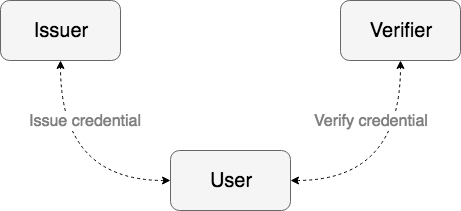
\includegraphics[scale=0.6]{images/CredentialSystemDiagram.png}
\caption{Overview of Credential System}
\label{fig: credential system overview}
\end{figure}

\noindent The \textbf{Credential} is an object with which the user may prove his qualities or entitlements, which may have following properties:
\begin{itemize}
    \item Does not reveal signed attributes to the verifying entity. 
    \item The verifier cannot link multiple presentations of the same credential.
    \item Can be issued under masked attributes (e.g. private keys, sensitive data etc.)
\end{itemize}

Description provided here should serve as general intuition of the system, more in-depth definitions and requirements will be provided in later parts of this paper. One should remember that although the formal definitions will build the cryptographic base of the system, the idea of what the system should do, and the motivation behind the need for such system, should be understood intuitively. 


\section{Use Cases}

Apart from the example from the introduction we can consider following scenarios:
\begin{itemize}
    \item \textbf{Room access system}
    
    Opening doors by presenting proper credential with possible option to make tracking users infeasible. Access rights and restrictions are naturally present in form of an attribute.
    \item \textbf{Bus ticket system}
    
    Verification does not require presentation of other IDs, and does not leak any information about communication patterns.
    \item \textbf{Online Movie Subscription}
    
    The only thing that gets verified is if one have valid subscription.
    \item \textbf{Driving license}
    
    Understood as driving permission ("this person is allowed to drive this kind of vehicle") without disclosing sensitive information.
\end{itemize}

The scenarios are endless and only on the need depend how they could be solved. The motivation of this paper is to equip the people in tools necessary to create such working and secure Credential System. The operational requirements of the system are presented in next section.


\section{System Requirements}
Below we present general requirements of the Credential System.

\begin{itemize}
    \item \textbf{Credential unforgeability}
    
    It should be infeasable for any number of colluding parties to obtain a valid credential without consent of the issuer.
    \item \textbf{Attributes privacy} 
    
    If should be infeasable for any number of colluding parties to obtain value of hidden attributes, without the owner reveling them.
    \item \textbf{Computational effectiveness}
    
    Performed computations should be possibly efficient and require small storage size without compromising security.
    \item \textbf{Transparency}
    
    System should be possibly simple and transparent from the user's perspective.
    \item \textbf{Modularity}
    
    System should be compact, extendable and ready for integration with similar existing systems.
\end{itemize}
Additionally, the system might provide:
\begin{itemize}
    \item \textbf{Multiple-show unlinkability}
    
    It should be infeasable for any number of colluding parties to link multiple presentations of the same credential. This considers only the attributes that are meant to be hidden. If we consider the case of linking users to the pseudonyms in domains it is natural to expect such possibility.
    
    \item \textbf{Non-transferability}
    
    It should be infeasable for any number of colluding parties to transfer a valid credential between different users without sharing all credential data (all or nothing).
\end{itemize}


% \section{Structure of this Document}
% In section ...
% In section

% What might be skipped and why
% What parts are the core of this document

\cleardoublepage
\chapter{Preliminaries}
\thispagestyle{chapterBeginStyle}


\section{Credential System Definitions}
To formalize the design process of credential system we state necessary definitions. At the end we present some examples to give proper intuition for used terms. 

\begin{definition}[Credential]
Credential is a statement, issued by an issuing entity, representing a relationship with the user (possibly based on some attributes). Credentials are presented to the verifying entities.
\end{definition}

\begin{definition}[Credential Type]
Credential type is a class of credentials representing the same statement with no relation to a user.
\end{definition}

\begin{example}[Driver's license]
\textbf{Statement:} "Owner is allowed to drive following vehicles: ... ".
\textbf{User:} Owner of the document. 
\textbf{Issuer:} Department of motor vehicles.
\textbf{Verifier:} e.g. Police (represented by a police officer). 
\textbf{Credential type:} "driving permission".
\end{example}

\begin{definition}[Credential System]
Credential system consists of three interacting parties: users, issuers and verifying entities. Such system must provide functionality for credential issuance and verification. Addition of new users and other entities should be possible.
\end{definition}

\begin{example}[Cinema ticket discounts for students]
In some cinemas there is a price discount for students. To obtain it one has to present valid student ID. In this scenario the university is the issuing entity (Note that there are more than one university) and the cinema is the verifier (represented by a worker selling tickets). It is important to notice that the verifying entity may be an issuer of another credential (cinema ticket), this gives natural flow to the whole system.
\end{example}

\begin{definition}[Non-transferable Credential]
A non-transferable credential is a credential that is uniquely associated with the owner and cannot be transferred to another user without transferring their identity.
\end{definition}

\begin{example}[Public transport]
There are many types of tickets one can buy in Wrocław. The one-time ticket is an example of transferable credential in the sense that one can give it to another person after validating it and it remains valid for that person (we do not consider here the question whether it is legal, only that it is possible). It is not bound to ones name.

But the monthly ticket is connected with the identity of the holder (name and photo) because it has to be encoded on Urban Card (electronic document for public communication in Wrocław). In this case one would have to share the "visual identity" (photo) with the other person.
\end{example}

\begin{definition}[Anonymous Credential System]
In anonymous credential system user upon presentation of credential to verifying entity reveals no other information than the fact that he is in possession of valid credential issued by a legitimate authority. It is infeasable for any party (or a colluding group of parties) to learn more about the user than he agreed to during credential presentation. Such system must provide functionality for:
\begin{enumerate}
    \item Issuance of credentials,
    \item Verification of credentials.
\end{enumerate}
\end{definition}

\begin{definition}[Pseudonymous Credential System]
Pseudonymous credential system is a sub-class of anonymous credential system in which a pseudonym is uniquely established between a user and an issuing (and, if required by system design, a verifying) organization. Issuers and verifying entities know users only by pseudonyms and it is infeasable for any party (or a colluding group of parties) to learn more about the user than he agreed to during credential presentation. Such system must provide functionality for:
\begin{enumerate}
    \item Registration with an organization (obtaining valid pseudonym),
    \item Issue of credentials for pseudonym,
    \item Transfer of credentials (between pseudonyms of the same user),
    \item Verification of credentials.
\end{enumerate}
\end{definition}

\begin{definition}[One-show Credential]
A one-show credential is a credential which may be presented only once by the owner without compromising the properties and security of the system. For subsequent presentations reissuing is required to preserve system properties.
\end{definition}

\begin{definition}[Multiple-show Credential]
A multiple-show credential is a credential which may be presented multiple times by the owner without compromising the properties and security of the system.
\end{definition}

\begin{definition}[PPT entities]
Each party in a credential system i.e users, issuers and verifiers, are probabilistic polynomial time Turing machines ($\textit{PPT}_{\textit{TM}}$) 
\end{definition}



\section{Cryptographic Assumptions}

% \begin{definition}[Notation]
% We will use elliptic curve notation of group operations. That is:
% \begin{itemize}
%     \item $(\Group, q, G)$ is a tuple of cyclic group or order $q$ with generator $G$,
%     \item $A, B \in \Group \quad A + B$ refers to point addition,
%     \item $A, B \in \Group \quad A - B$ refers to point subtraction,
%     \item $x \in \ZZ_q, A \in \Group \quad [x]G$ refers to point multiplication.
% \end{itemize}
% In other cases we will also refer to integer field notation of point exponentiation, but assuming its ordinarity the detailed description will be ommited. 
% \end{definition}

\begin{assumption}[Discrete Logarithm (DL)]
The discrete logarithm problem is hard relative to $\setup$ if for all \textsc{PPT} algorithms \adv
% the following is negligible:
$$\prob{(\Group, q, g) \gets \setup(\secparam); h \gets \Group; x \gets \adv(\Group, q, g, h): g^x = h} \leq \varepsilon $$
for a negligible $\varepsilon$. 
The discrete logarithm assumption is that there exists $\setup$ relative to which the discrete logarithm problem is hard.
\end{assumption}

\begin{assumption}[Discrete Logarithm Relation]
The discrete logarithm relation problem is hard relative to $\setup$ if for all \textsc{PPT} algorithms \adv
% the following is negligible:
$$\prob{(\Group, q) \gets \setup(\secparam); g_1, \dots g_n \sample \Group; a_1, \dots a_n \gets \adv(\Group, q, g_1, \dots g_n): \exists a_i \neq 0 \wedge \prod_{i=1}^n g_i^{a_i} = 1} \leq \varepsilon $$
for a negligible $\varepsilon$. 
We say $\prod_{i=1}^n g_i^{a_i} = 1$ is a non trivial discrete logarithm relation between $g_1, \dots g_n$. 
The discrete logarithm relation assumption is that it is infeasable to find non-trivial relation between randomly chosen group elements. For $n \geq 1$ this is equivalent to the discrete logarithm assumption.
\end{assumption}

\begin{assumption}[Computational Diffie-Hellman (CDH)]
The computational Diffie-Hellman problem is hard relative to $\setup$ if for all \textsc{PPT} algorithms \adv
$$\prob{(\Group, q, g) \gets \setup(\secparam); a, b \sample \ZZ_q; g^{ab} \gets \adv(\Group, q, g, g^a, g^b)} \leq \varepsilon$$
for a negligible $\varepsilon$.
The computational Diffie-Hellman assumption is that there exists $\setup$ relative to which the computational Diffie-Hellman problem is hard.
\end{assumption}

\begin{assumption}[Decisional Diffie-Hellman (DDH)]
The decisional Diffie-Hellman problem is hard relative to $\setup$ if for all \textsc{PPT} algorithms \adv
$$ \abs{ \prob{\text{True} \gets \adv(\Group, q, g, g^a, g^b, g^{ab})} - \prob{\text{True} \gets \adv(\Group, q, g, g^a, g^b, g^c)} } \leq \varepsilon $$
for a negligible $\varepsilon$, 
where $(\Group, q, g) \gets \setup(\secparam)$, and $a, b, c \sample \ZZ_q$.

The decisional Diffie-Hellman assumption is that there exists $\setup$ relative to which the decisional Diffie-Hellman problem is hard.
\end{assumption}

% \begin{definition}[Bilinear Maps]
% Suppose that $\setup(\secparam)$ outputs the setup for $(\Group, +)$ with generator $G$ and $(\Group_T, \cdot)$ with generator $\widetilde G$, such that $\abs{\langle G \rangle} = \abs{\langle \widetilde G \rangle} = q$ where $q$ is prime. Let $e: \Group \times \Group \rightarrow \Group_T$ be be a function such that:
% \begin{enumerate}
%     \item (Bilinear) $(\forall A, B \in \Group)(\forall x, y \in \ZZ_q) \quad e([x]A, [y]B) = e(A, B)^{xy}$.
%     \item (Non-degenerate) $\exists P, Q \in \Group$ s.t. $e(P,Q) \neq 1$, where $1$ is the identity of $G_T$.
%     \item (Efficient) There exists an efficient algorithm for computing $e$.
% \end{enumerate}
% We write: $(q, \Group, G, \Group_T, \widetilde G, e) \gets \setup(\secparam)$.
% \end{definition}
% Note, that because $e([a]G, [b]G) = e(G, G)^{ab} = e(G, [ab]G)$ holds in groups with bilinear pairings, the Decisional Diffie-Hellman problem is easily solved in such groups.

\begin{definition}[Bilinear Maps]
Let $(q, \Group_1, \Group_2, \Group_T, e) \gets \setup(\secparam)$, such that $\Group_1$ and $\Group_2$ are two additive cyclic groups of order $q$. We say that $e$ is a bilinear map, if for multiplicative group $\Group_T$, $e: \Group_1 \times \Group_2 \rightarrow \Group_T$ such that:
\begin{enumerate}
    \item (Bilinear) $(\forall A, B \in \Group)(\forall x, y \in \ZZ_q) \quad e([x]A, [y]B) = e(A, B)^{xy}$.
    \item (Non-degenerate) $\exists P, Q \in \Group$ s.t. $e(P,Q) \neq 1$, where $1$ is the identity of $G_T$.
    \item (Efficient) There exists an efficient algorithm for computing $e$.
\end{enumerate}
\end{definition}

\begin{definition}[Type 1 Pairing]
We say, that a bilinear pairing is a Type 1 Pairing, if $\Group_1 = \Group_2$.
\end{definition}

\begin{definition}[Type 2 Pairing]
We say, that a bilinear pairing is a Type 2 Pairing, if $\Group_1 \neq \Group_2$, but there exists an efficiently computable homomorphism $\phi: \Group_1 \rightarrow \Group_2$.
\end{definition}

\begin{definition}[Type 3 Pairing]
We say, that a bilinear pairing is a Type 3 Pairing, if $\Group_1 \neq \Group_2$, and there are no efficiently computable homomorphisms from $\Group_1 \rightarrow \Group_2$.
\end{definition}
Note, that in type 1 and 2 pairings Decisional Diffie-Hellman problem is easily solved. Because $e([a]G_1, [b]G_2) = e(G_1, G_2)^{ab} = e(G_1, [ab]G_2)$.

\begin{assumption}[LRSW assumption \cite{pseudonym-systems}] \label{def:lrsw}
Let $(q, \Group, G) \gets \setup(\secparam)$. Let $A = [a]G, B = [b]G \in \Group$. Let $O_{A, B}(\cdot)$ be an oracle that on input $m \in \ZZ_q$ outputs $(R, [b]R, [a + mab]R)$ for a randomly chosen $R \in \Group$. Then for all \textsc{PPT} algorithms \adv, the following is negligible:
\begin{multline*}
\prob{} \Big[ (m, X, Y, Z) \gets \adv^{O_{A, B}} (q, \Group, G, A, B): \\ 
m \notin Q \wedge m \in \ZZ_q \wedge m \neq 0 \wedge X \in \Group \wedge Y = [b]X \wedge Z = [a + mab]X \Big] \leq \varepsilon
\end{multline*}
for a negligible $\varepsilon$, where $Q$ is the set of previous queries that $\adv$ made to $O_{A, B}(\cdot)$.
\end{assumption}


\section{Chosen Cryptographic Primitives}

% \subsection{Zero-Knowledge Proof of Knowledge (ZKP)}
\begin{definition}[Zero-Knowledge Proof of Knowledge (ZKP)]
A zero-knowledge proof of knowledge is a protocol between two \textsc{PPT} entities called Prover and Verifier. The Prover proves to the verifier that he knows a set of values without revealing these values. 

We use notation introduced by Camenish and Stadler \cite{cs-notation-zkp} for various proofs of knowledge. For instance,
$$\textit{ZKP } \set{ (\alpha, \beta, \gamma): y = g^\alpha h^\beta \wedge \widetilde y = \widetilde g^\alpha \widetilde h^\gamma \wedge (u \leq \alpha \leq v) }$$
denotes a "zero-knowledge" Proof of Knowledge of values $\alpha, \beta$ and $\gamma$ such that $y = g^\alpha h^\beta$ and $\widetilde y = \widetilde g^\alpha \widetilde h^\gamma$ holds, where $u \leq \alpha \leq v$", where $y, g, h, \widetilde y, \widetilde g$ and $\widetilde h$ are elements of some groups $\Group = \langle g \rangle = \langle h \rangle$ and $\widetilde \Group = \langle \widetilde g \rangle = \langle \widetilde h \rangle $. Greek letters denote quantities the knowledge of which is being proved, while all other parameters are known to the verifier.
\end{definition}

% \subsection{Signature Scheme}
\begin{definition}[Signature Scheme]
A signature scheme consists of three \textsc{PPT} algorithms $(\kgen, \sig, \verify)$ such that:
\begin{itemize}
    \item The key generation algorithm $\kgen$, takes as input a security parameter $\secpar$ and outputs a pair of keys $(\sk, \pk)$. These are called secret key and public key respectively.
    \item The signature algorithm $\sig$, which produces a signature $\sigma$ using private key and message $m$ from a message space. We write this as $\sigma \gets \sig_{sk}(m)$.
    \item The verification algorithm $\verify$, which tests whether $\sigma$ is a valid signature for message $m$ using public key $\pk$. That is $b \gets \verify_\pk(m, \sigma)$ where $b \in \set{0, 1}$ and $b = 1$ if and only if the signature is valid.
\end{itemize}
\end{definition}


% \subsection{Commitment Scheme}
\begin{definition}[Commitment Scheme]
A non-interactive commitment scheme consists of two \textsc{PPT} algorithms $(\setup$, $\commit)$ such that:
\begin{itemize}
    \item The setup algorithm $\setup$, which takes as input a security parameter $\secparam$ and outputs public parameters for the scheme.
    \item The commitment algorithm $\commit$, which defines a function $M \times R \rightarrow C$ for message space $M$, randomness space $R$ and commitment space $C$ determined by public parameters. $(\com = \commit(m, r))$.
\end{itemize}
% For a message $m \in M$ the algorithm samples $r \sample R$ uniformly at random, and computes commitment $\com = \commit(m, r)$.
\end{definition}

\begin{definition}[Hiding Commitment]
A commitment scheme is hiding if for all \textsc{PPT} algorithms $\adv$
\begin{multline*}
  \Bigg| \prob{} \Big[ (M, R, C) \gets \setup(\secparam); \\ m_0, m_1 \in M; b \sample \bin; r \sample R; \com = \commit(m_b, r);
  b' \gets \adv(M, R, C, \com): b = b' \Big] - \frac{1}{2} \Bigg| \leq \varepsilon
\end{multline*}
for a negligible $\varepsilon$. If it is equal to $0$ then we say the scheme is perfectly hiding.
\end{definition}

\begin{definition}[Binding Commitment]
A commitment scheme is binding if for all \textsc{PPT} algorithms $\adv$
$$ \prob{} \Big[ (M, R, C) \gets \setup(\secparam); m_0, m_1 \in M; r_0, r_1 \in R: \commit(m_0, r_0) = \commit(m_1, r_1) \wedge m_0 \neq m_1 \Big] \leq \varepsilon $$
for a negligible $\varepsilon$. If it is equal to $0$ then we say the scheme is perfectly binding.
\end{definition}

\section{Chosen Cryptographic Protocols}

% \subsection{Pedersen Commitment}
% As in \cite{pedersen-commitment}.
\begin{definition}[Pedersen Commitment \cite{pedersen-commitment}]
Defining public parameters $M, R = \ZZ_q, C = \Group$.
\begin{itemize}
    \item[] $\setup: H, G \sample \Group$ such that nobody knows $\log_G(H)$ or $\log_H(G)$.
    \item[] $\commit(m, r) = [r]H + [m]G$  
\end{itemize}
\end{definition}

% \subsection{Pedersen Vector Commitment}
\begin{definition}[Pedersen Vector Commitment]
Defining public parameters $M = \ZZ_q^n, R = \ZZ_q, C = \Group$.
\begin{itemize}
    \item[] $\setup: (G_0, G_1, \dots G_n) \sample \Group$ such that nobody knows $\log_{G_i}(G_j)$ for any $i, j \in \set{0, \dots n}$.
    \item[] $\commit((m_1, \dots, m_n), r) = [r]G_0 + \sum_{i=1}^n [m_i]G_i$
\end{itemize}
\end{definition}
The Pedersen vector commitment is perfectly hiding and computationally binding under the discrete logarithm assumption. We might also set $r = 0$, in which case the commitment is binding but not hiding.


% \subsection{Okamoto-Schnorr Protocol}
\begin{definition}[Okamoto-Schnorr Protocol]
Okamoto-Schnorr protocol \cite{Schnorr1991, okamoto} was designed as zero-knowledge identification scheme, which may be used as a realization of 
$$ ZKP\set{(\alpha, \beta): s = g^\alpha \cdot h^\beta} $$
It can be further extended to obtain proof for $n$ values:
$$ ZKP\set{(\alpha_1, \alpha_2, \dots, \alpha_n): s = g_1^{\alpha_1} \cdot g_2^{\alpha_2} \cdot \dots g_n^{\alpha_n}} $$
On figure \ref{fig:schnorr} we recall the original scheme, secure under discrete logarithm assumption.
\end{definition}
Note, that one can use Okamoto-Schnorr to proof the knowledge opening of the Pedersen and Vector Pedersen Commitment, this construction will be used in the future. 

\begin{figure}[h]
\centering

\begin{pcvstack}

\begin{pchstack}[center]
\procedure[linenumbering, width=5cm]{$\Setup(\secpar)$}{%
 (\Group, q, g_1, g_2) \gets \setup(\secparam) \\
 \pcreturn (\Group, q, g_1, g_2)
}

\pchspace

\procedure[linenumbering, width=5cm]{$\kgen(\Group, q, g_1, g_2)$}{%
 \alpha, \beta \sample \ZZ_q \\
 s = g_1^{-\alpha} g_2^{-\beta} \\
 \pk = s \\
 \sk = (\alpha, \beta) \\
 \pcreturn (\sk, \pk)
}

\end{pchstack}

\pcvspace

\procedure[width=11cm]{$\pcalgostyle{Proof}(\alpha, \beta)$}{%
  \textbf{Prover } (g_1, g_2, \alpha, \beta) \> \> \textbf{Verifier } (g_1, g_2, s)\\
  r_1, r_2 \sample \ZZ_q \> \> \\
  t = g_1^{r_1}g_2^{r_2} \> \> \\
  \> \sendmessageright*[3.5cm]{t} \> \\
  \> \> c \sample \ZZ_q \\
  \> \sendmessageleft*[3.5cm]{c} \> \\
  x_1 = r_1 + c \cdot \alpha \> \> \\
  x_2 = r_2 + c \cdot \beta \> \> \\
  \> \sendmessageright*[3.5cm]{x_1, x_2} \> \\
  \> \> t \stackrel{?}{=} g_1^{x_1}g_2^{x_2}s^c
}
\end{pcvstack}

\caption{Okamoto-Schnorr Identification Protocol}
\label{fig:schnorr}
\end{figure}


\cleardoublepage
\chapter{Credential System Protocols}
\thispagestyle{chapterBeginStyle}

\section{Solution}
Or design of Credential System aims to be possibly computationally efficient. We focus on the construction based on elliptic cures with bilinear pairings instead of the earlier work of Camenisch and Lysyanskaya \cite{anoncreds-rsa} which was based on the RSA assumption that is rather computationally expensive.

We use Anonymous Credential from Bilinear Maps by Camenisch and Lysyanskaya \cite{anon-creds-cl04} as the backbone for out design. We also decided to opt for the more efficient verification protocol introduced by Słowik and Wszoła \cite{slowik-efficient-cl-lrsw} due to its computational cost reduction on client side of protocol. In last section we present construction by Bobowski and Słowik \cite{complexity-reduction-bobowski}, that efficiently reduces computational cost of verification even further by reducing number of required pairing operations.

We will omit the proofs of security of those protocols and refer to the original papers. We will focus and extend the analysis that is focused on possible practical applications for the credential system design. 

\begin{remark}[Credential System]
Credential system, as stated by Camenisch and Lysyanskaya \cite{signature-scheme-with-efficient-protocols}, is sufficient to exhibit a commitment scheme, a signature scheme, and efficient protocols for:
\begin{itemize}
    \item proving equality of two committed values,
    \item signing a committed value (without revealing this value to the signer), and
    \item proving the knowledge of a signature on a committed value.
\end{itemize}
\end{remark}


\section{Background Security Assumptions}
For the model of credential system we assume that:
\begin{itemize}
    \item the security of transport layer for the exchanged messages, and
    \item existence of some PKI, in the most general form, for the certificate verification.
    \item \textit{(optional) in case of pseudonymous system, we assume that the protocols of establishing a pseudonym (understood as set of attributes with domain private key) exists. }
\end{itemize}
We do not consider here which protocols and schemes achieve those requirements, we operate on higher level of abstraction.


% \section{Commitment Schemes}

% \begin{definition}[Exponent Commitment Scheme]
% Let $G \in \Group$. The commitmer commits himself to an $s \in \ZZ_q$ by computing
% $$ C = [s]G $$
% Such commitment can later be opened by revealing $s$. $C$ reveals no information about $s$, and the commiter cannot open a commitment to $s$ as $s' \neq s$. It is hiding and binding under discrete logarithm assumption.
% \end{definition}

% \begin{definition}[Pedersen Commitment Scheme \cite{pedersen-commitment}]
% Let $H, G \in \Group$ such that nobody knows $\log_G(H)$ or $\log_H(G)$. The committer commits himself to an $s \in \ZZ_q$ by choosing $t \in \ZZ_q$ at random and computing
% $$ C = [t]H + [s]G$$
% Such commitment can later be opened by reveling $s$ and $t$. $C$ reveals no information about $s$, and the committer cannot open a commitment to $s$ as $s' \neq s$ unless he knows $\log_G(H)$ or $\log_H(G)$. For any $s \in \ZZ_q$ and for randomly uniformly chosen $t \in \ZZ_q$, $C$ is uniformly distributed in $\Group$. It is information-theoretically hiding, and is binding under discrete logarithm assumption.
% \end{definition}

% \begin{definition}[Sum Commitment Scheme]
% Sum commitment scheme is a natural extension of Pedersen commietment scheme. \newline
% Let $(G_0, G_1, \dots G_n) \in \Group$ such that nobody knows $\log_{G_i}(G_j)$ for any $i, j \in \set{0, \dots n}$. The committer commits himself to $\set{s_i} \in \ZZ_q^n$ by choosing $t \in \ZZ_q$ at random and computing
% $$ \textstyle C = [t]G_0 + \sum_{i=1}^n [s_i]G_i $$
% Such commitment can later be opened by reveling $\set{s_i}$ and $t$. $C$ reveals no information about $\set{s_i}$, and the committer cannot open a commitment to $\set{s_i}$ as $\set{s'_i} \neq \set{s_i}$ unless he knows any $\log_{G_i}(G_j)$. For any $\set{s_i} \in \ZZ_q^n$ and for randomly uniformly chosen $t \in \ZZ_q$, $C$ is uniformly distributed in $\Group$. It is information-theoretically hiding, and is binding under discrete logarithm assumption.
% \end{definition}

% \begin{remark}[ZKP for Committments]
% Note that for presented commitments we can easily construct the Zero-knowledge proof of knowledge by employing the Okamoto-Schnorr protocol.
% \end{remark}

% \begin{remark}[Information-Theoretically Hiding]
% The key difference between Pedersen and Exponent commitment schemes is in information-theoretically hiding property.
% It can be intuitively understood as the problem of linking committed values between different protocol executions. In Pederson such linking is infeasable because there are $q$ possible commitments $C$ for the same $s$ and each with the same probability, where exponent commitment is always the same.
% \end{remark}

\section{Signature Scheme}
We now present construction of CL-LRSW randomizable signatures (figure \ref{fig:cl-lrsw}) presented by Camenisch and Lysyanskaya \cite{anon-creds-cl04}. The signatures are based on LRSW Assumption \cite{pseudonym-systems}. We consider the asymmetric pairing and for notation clarity all variables are implicitly from $\Group_1$, unless other wise stated in the variable index. 


\begin{figure}[htp]
\centering

\begin{pcvstack}

\begin{pchstack}
\procedure[linenumbering, width=7cm]{$\Setup(\secpar)$:}{%
  \text{$(q, \Group_1, \Group_2, \Group_T, e) \gets \setup(\secparam)$}  \\
  \pcreturn (q, \Group_1, \Group_2, \Group_T, e)
}

\pchspace

\procedure[linenumbering, width=7cm]{$\kgen(l)$:}{%
  (x, y, z_1, \dots, z_l) \sample \ZZ_q^{l+2} \\
  X^{(2)} := [x]G_2 \\
  Y^{(2)} := [y]G_2 \\
  Z^{(2)}_i := [z_i]G_2 \quad i \in \set{1, \dots l}\\
  Z_i := [z_i]G_1 \quad i \in \set{1, \dots l}\\
  \sk := (x, y, z_1, \dots, z_l) \\
  \pk := (X^{(2)}, Y^{(2)}, Z^{(2)}_1, \dots Z^{(2)}_l, Z_1, \dots Z_l) \\
  \pcreturn (\sk, \pk)
}
\end{pchstack}

\pcvspace

\begin{pchstack}
\procedure[linenumbering, width=7cm]{$\sig_\sk((m_0, \dots m_l) \in \ZZ_q^{l+1})$:}{%
  \sk = (x, y, z_1, \dots z_l) \\
  A_0 \sample \Group_1 \\
  B_0 := [y]A_0 \\
  \pcfor i \in \set{1, \dots l} \pcdo \\
  \pcind A_i := [z_i]A_0 \\
  \pcind B_i := [z_i]B_0 \\
  C := [x]A_0 + \textstyle \sum_{i=0}^l [xym_i]A_i \\
  \sigma := (A_0, \dots A_l, B_0, \dots B_l, C) \\
  \pcreturn \sigma
}

\pchspace

\procedure[linenumbering, width=7cm]{$\sig_\sk(M \in \Group)$:}{%
  \sk = (x, y, z_1, \dots z_l) \\
  \alpha \sample \ZZ_q \\
  A_0 := [\alpha]G_1 \\
  B_0 := [y]A_0 \\
  \pcfor i \in \set{1, \dots l} \pcdo \\
  \pcind A_i := [z_i]A_0 \\
  \pcind B_i := [z_i]B_0 \\
  C := [x]A_0 + [\alpha xy]M \\
  \sigma := (A_0, \dots A_l, B_0, \dots B_l, C) \\
  \pcreturn \sigma
}
\end{pchstack}

\pcvspace

\procedure[linenumbering, width=9cm]{$\verify(\sigma, (m_0, \dots, m_l) \in \ZZ_q^{l+1})$:}{%
  \pk = (X^{(2)}, Y^{(2)}, Z^{(2)}_1, \dots Z^{(2)}_l, Z_1, \dots Z_l) \\
  \sigma = (A_0, \dots A_l, B_0, \dots B_l, C) \\
  \pcif e(A_0, Y^{(2)}) \neq e(B_0, G_2) \pcthen \\
  \pcind \pcreturn \pcfalse \\
  \pcfor i \in \set{1, \dots l} \pcdo \\
  \pcind \pcif e(A_0, Z^{(2)}_i) \neq e(A_i, G_2) \pcthen \\
  \pcind \pcind \pcreturn \pcfalse \\
  \pcind \pcif e(A_i, Y^{(2)}) \neq e(B_i, G_2) \pcthen \\
  \pcind \pcind \pcreturn \pcfalse \\
  \pcreturn e(C, G_2) \stackrel{?}{=} e(A_0, X^{(2)}) \textstyle \prod_{i=0}^l e([m_i]B_i, X^{(2)})
}

\end{pcvstack}

\caption{CL-LRSW signature algorithms}
\label{fig:cl-lrsw}
\end{figure}

Presented scheme has many useful (for credential system) properties. This scheme allows to:
\begin{itemize}
  \item sign $l+1$ messages into one batch,
  \item obtain signature on hidden values $(\sig_\sk(M \in \Group))$,
  \item re-randomize the signature for each presentation,
  \item proof validity of signature without revealing hidden values in the interactive protocol, and
  \item create signature such that even computationally unbound issuer cannot learn the values (thanks to Pedersen commitment scheme).
\end{itemize}


\begin{remark}[Flexibility of Commitment Composition]
Let us denote $Z_0 = G$, then the commitment $M$ can be represented as
$$ M = \textstyle \sum_{i=0}^l [m_i]Z_i $$
Let us consider multiple scenarios of calculating this sum between the user and issuer.
\begin{itemize}
    \item \textbf{Open}
    
    User sends $m = \set{m_i}$ messages in plain-text to the issuer, then issuer can calculate the sum on its side $ M = \sum_{i=0}^l [m_i]Z_i $.
    \item \textbf{Exponent}
    
    User sends $M_i = \set{[m_i]Z_i}$. Issuer: $M = \sum_{i=0}^l M_i$.
    \item \textbf{Pedersen}
    
    User sends $M_i = \set{[r_i]G + [m_i]Z_i}$ for $i \in \set{1, \dots l}$, where $r_i \sample \ZZ_q$. Issuer combines $M = \sum_{i=0}^l M_i$ (Note that if we define $m_0 = \sum_{i=1}^l r_i$ then the scheme closely resembles the Vector commitment, but user still has to remember all $r_i$).
    \item \textbf{Vector}
    
    User calculates $ M = \sum_{i=0}^l [m_i]Z_i $ (Note, that if information-theoretically hiding is desired, at least one of $\set{m_i}$ messages has to be a random value). Issuer does nothing.
\end{itemize}
\end{remark}
% We are not bound to calculate the sum in only one of presented ways, we can combine those based on the needs and requirements. For example, when buying a beer the date of birth can be send in Pedersen commitment and other attributes (e.g. domain keys) will be sent in sum. This issuer's required commitments can be described as set $\set{\text{pedersen}, \text{sum}}$. 

% \begin{remark}[Information-Theoretically Hiding Commitment]
% In the theory part of this document we do not consider every case of possible usage, but rather describe what should be done to achieve certain properties. That is, if one wants to obtain theoretically-hiding property of commitment in the Pedersen Vector commitment, one has to add the randomizing message (e.g. $m_0 \sample \ZZ_q$).
% \end{remark}


\begin{corollary}[Generalized Commitment Composition]
Let $\set{Z_i}_{i=0}^l$ denote public key of the issuer, where $Z_0 = G$.
Let $\set{m_i}$ be the set of $l + 1$ messages, $v, p, e, o$ are sets of indices $(v \cup p \cup e \cup o = \set{0, \dots l})$ that are to be committed in vector, pedersen, exponent and open commitment. The combined calculations of message commitment can be calculates as follows.

\begin{figure}[H]
\centering
\procedure{}{%
  \textbf{User} \< \< \textbf{Issuer}\\
  \textstyle V = \sum_{i \in v} [m_i]Z_i\< \< \\
  P = \set{[r_i]G + [m_i]Z_i}_{i \in p} \quad r_i \sample \ZZ_q \< \< \\
  E = \set{[m_i]Z_i}_{i \in e} \< \< \\
  O = \set{m_i}_{i \in o} \< \< \\
  \< \sendmessageright*[3.5cm]{v, V, p, P, e, E, o, O} \< \\
  \< \< \textstyle M = V + \sum P + \sum E + \sum_{i \in o} [O_i]Z_i \\
}
\caption{Generalized Commitment Composition}
\label{proto:generalized-commitment-composition}
\end{figure}
\end{corollary}

\begin{remark}[Issuer-Dependent ZKP on Commitments]
Division of $M$ into separate commitments and plain-text messages allows to construct the issuer-dependent zero-knowledge proofs of knowledge on chosen attributes, e.g. perform range proof for numerical values (Range proofs \cite{bulletproofs}). Here we only acknowledge the possibility and leave the design of such extensions for future work.
\end{remark}

Though the division of commitment $M$ into $(V, P, E, O)$ has its benefits, in following sections we will assume that only Pedersen Vector commitment is used for all values (represented as $M$). We hope that such a shortcut will result in more compact description of theory of the system, and previously presented constructions will give proper intuition of how to possibly employ other commitment schemes.

% \section{Attributes List Convention}
% Because the attributes list differs from issuer to issuer there emerges the need to somehow organize the structure of set $\set{m_i}$. In this, theoretical part, we will only give the overview (an intuition). The more structured and practical approach to attributes organization will be found in practical part of the document.

% \begin{assumption}[Knowledge of Attributes List]
% We assume that the user has the list of required attributes and its description, that is, knows which attributes are awaited and in what commitment schemes.
% \end{assumption}
% Now we will briefly enumerate through some of the possible requirements of $\set{m_i}$.

% \begin{requirement}[Sum Commitment]
% If the sum commitment is used, it is required that the $m_0 \sample \ZZ_q$. It serves the role of the randomizer that is required to achieve information-theoretically hiding commitment.
% \end{requirement}

% \begin{requirement}[Pedersen Commitment]
% If the Pedersen commitment is used, it is required that each $m_j \sample \ZZ_q$. It serves the role of the randomizer that is required to achieve information-theoretically hiding commitment.
% \end{requirement}

% \begin{requirement}[Non-transferable credential]
% If the credential is to be non-transferable, then there exists some private value $m_x$ that is the identity of the user i.e. passing it to the other user compromises the security of owners data. 
% \end{requirement}

% % m_0
% % m_1 - sk
% % strings -> hash
% % standarization


% \section{Access Certificates}
% % todo

\section{Obtaining a Signature on a Committed Value}
Suppose that $M = [m_0]G + \sum_{i=1}^l [m_i]Z_i$ is a Pedersen vector commitment to set of messages $(m_0, \dots m_l)$ whose signature the user wishes to obtain (remember that if the information-theoretically hiding property is desired then one of messages has to be sampled at random). Then, the user gives a zero-knowledge proof of knowledge of the opening of the commitment:
$$ \textstyle \textit{ZKP } \set{(\mu_0, \dots \mu_l): M = [\mu_0]G + \sum_{i=1}^l [\mu_i]Z_i} $$
After this step there is a possible extension of the protocol of further checks (range check etc.), depending on needs and requirements. At last, the issuer computes the signature $\sigma = (\set{A_i}, \set{B_i}, C)$ and sends credential to the user.

The protocol is depicted on figure \ref{proto:cred-issue}.

\begin{figure}[p]
\centering
\procedure{$\pcalgostyle{Issue}(m)$}{%
  \textbf{User} \< \< \textbf{Issuer}\\
  \pk_I = \Big( X^{(2)}, Y^{(2)}, \set{Z^{(2)}_i}, \set{Z_i} \Big) \< \< \pk_I = \Big( X^{(2)}, Y^{(2)}, \set{Z^{(2)}_i}, \set{Z_i} \Big) \\
  m = (m_0, \dots m_l) \< \< \sk_I = (x, y, z_1, \dots z_l) \pclb
  \pcintertext[dotted]{Attributes commitment}
  M = [m_0]G + \textstyle \sum_{i = 1}^l [m_i]Z_i \< \< \\
  \< \sendmessageright*[3cm]{M} \< \pclb
  \pcintertext[dotted]{ZKP of commitment opening} 
  k_i \sample \ZZ_q \quad \forall i \in \set{0, \dots l} \< \< \\
  T = [k_0]G + \textstyle \sum_{i = 1}^l [k_i]Z_i \< \< \\
  \< \sendmessageright*[3cm]{T} \< \\
  \< \< c \sample \ZZ_q \\
  \< \sendmessageleft*[3cm]{c} \< \\
  s_i = k_i - cm_i \quad \forall i \in \set{0, \dots l} \< \< \\
  \< \sendmessageright*[3cm]{s_0, \dots, s_l} \< \\
  \< \< T \stackrel{?}{=} \textstyle [c]M + [s_0]G + \sum_{i = 1}^l [s_i]Z_i \pclb
  \pcintertext[dotted]{CL-LRSW signature creation}
  \< \< \sigma = \sig_{sk_I}(M) \\
  \< \sendmessageleft*[3cm]{\sigma} \< \\
  \text{Store }(\sigma, (m_0, \dots m_l)) \< \< 
}
\caption{Credential Issuance Protocol}
\label{proto:cred-issue}
\end{figure}

% \begin{figure}[p]
% \centering
% \procedure{$\pcalgostyle{Issue}(m)$}{%
%   \textbf{User} \< \< \textbf{Issuer}\\
%   \pk_I = (X, Y, Z_1, \dots Z_l) \< \< \pk_I = (X, Y, Z_1, \dots Z_l) \\
%   m = (m_1, \dots m_l) \< \< \sk_I = (x, y, z_1, \dots z_l) \\
%   P - \text{set of public attributes indices} \< \< \\
%   H = \set{0, \dots l} \setminus  P \< \< \\
%   m_0 \sample \ZZ_q \< \<  \pclb
%   \pcintertext[dotted]{Public and hidden attributes}
%   m_P = (m_i : i \in P) \< \< \\
%   M_H = [m_0]G + \textstyle \sum_{i \in H \setminus \set{0}} [m_i]Z_i \< \< \\
%   \< \sendmessageright*[2.5cm]{P, m_p, M_H} \< \pclb
%   \pcintertext[dotted]{ZKP on hidden attributes} 
%   k_i \sample \ZZ_q \quad \forall i \in H \< \< \\
%   T = [k_0]G + \textstyle \sum_{i \in H \setminus \set{0}} [k_i]Z_i \< \< \\
%   \< \sendmessageright*[2.5cm]{T} \< \\
%   \< \< c \sample \ZZ_q \\
%   \< \sendmessageleft*[2.5cm]{c} \< \\
%   s_i = k_i - cm_i \quad \forall i \in H\< \< \\
%   \< \sendmessageright*[2.5cm]{\set{s_i}_{i \in H}} \< \\
%   \< \< [c]M_H + [s_0]G +\textstyle \sum_{i \in H \setminus \set{0}} [s_i]Z_i \stackrel{?}{=} T \pclb
%   \pcintertext[dotted]{LRSW signature creation}
%   \< \< M = M_H + \textstyle \sum_{i \in P} [m_i]Z_i \\
%   \< \< \sigma = \sig_{sk_I}(M) \\
%   \< \sendmessageleft*[2.5cm]{\sigma} \< \\
%   \text{Store }(\sigma, (m_0, \dots m_l)) \< \< 
% }
% \caption{Credential Issuance Protocol}
% \label{proto:cred-issue}
% \end{figure}

\section{Proving Knowledge of Signature}

The user computes a blinded version of the signature $\sigma$ and presents it to the verifier. Then, proves the knowledge of the signed message.
$$ \textstyle \textit{ZKP } \set{(\rho, (\mu_0, \dots \mu_l) ): \verify_\pk (\rho, (\mu_0, \dots \mu_l) ) = \text{True} }$$
Due to its efficiency and versatility we use the verification procedure designed by Słowik \& Wszoła   \cite{slowik-efficient-cl-lrsw} with employed Change-Base step construction, that can be used for future specialized value checks. The protocol is depicted on figure \ref{proto:cred-verify}, the steps of Change-Base are in in boxes.

We briefly state the corollary of Change-Base for our construction.
\begin{corollary}[Change-Base Step]
Assume that we have a set of indexed exponents $L$ and set of bases $\bigcup_{i \in L} \set{Q_i}$.
We can easily and very efficiently extend the verification protocol to check if the commitment $D = \sum_{i \in L} [m_i]Q_i$ was calculated properly using messages from signed credential.

User publishes the commitment $D$, and $t = [k_r]D + \sum_{i \in L} [-k_i] Q_i$.

Verifier checks the equality $t \stackrel{?}{=} [s_r]D + \sum_{i \in L} [-s_i] Q_i$ using the same $\set{s_i}$ from response phase.

\end{corollary}
The desired property of this step is that user can present some values in hidden form and proof that they are calculated properly (i.e. that user in fact knows those values). This committed form is meant to be later used for the specialized value checks (e.g. range proofs \cite{bulletproofs}), but this topic is not covered in this version of document and is left for future work. 



\begin{figure}[p]
\centering
\procedure{$\pcalgostyle{\verify}((\sigma, m))$}{%
  \textbf{User} \< \< \textbf{Verifier}\\
  \pk_I = \Big( X^{(2)}, Y^{(2)}, \set{Z^{(2)}_i}, \set{Z_i} \Big) \< \< \pk_I = \Big( X^{(2)}, Y^{(2)}, \set{Z^{(2)}_i}, \set{Z_i} \Big) \\
  \dbox{$\textstyle Q_L = \bigcup_{i \in L} \set{Q_i}$}\< \< \dbox{$\textstyle  Q_L = \bigcup_{i \in L} \set{Q_i} $} \\
  \sigma = (A_0, \dots A_l, B_0, \dots B_l, C) \< \< \\
  m = (m_0, \dots m_l) \< \< \pclb
  \pcintertext[dotted]{Signature blinding} 
  r, r' \sample \ZZ_q^2 \< \< \\
  \widetilde A_i = [r']A_i \quad \forall i \in \set{0, \dots l} \< \< \\
  \widetilde B_i = [r']B_i \quad \forall i \in \set{0, \dots l} \< \< \\
  \widetilde C = [rr']C \< \< \\
  \sigma' = (\widetilde A_0, \dots \widetilde A_l, \widetilde B_0, \dots \widetilde B_l, \widetilde C) \< \< \\
  \dbox{$\textstyle D = \sum_{i \in L} [m_i]Q_i$} \< \< \\
  \< \sendmessageright*[3cm]{\sigma' \dbox{$, D$}} \< \pclb
  \pcintertext[dotted]{ZKP of signed messages and randomizer $r$}
  k_r, k_0, \dots k_l \sample \ZZ_q^{l+2} \< \< \\
  T = [k_r]\widetilde A_0 + \textstyle \sum _{i = 0} ^ l [k_i]\widetilde B_i \< \< \\
  \dbox{$\textstyle t = [k_r]D + \sum_{i \in L} [-k_i] Q_i$} \< \< \\
  \< \sendmessageright*[3cm]{T \dbox{$, t$}} \< \\
  \< \< c \sample \ZZ_q \\
  \< \sendmessageleft*[3cm]{c} \< \\
  s_r = k_r - cr \< \< \\
  s_i = k_i - crm_i \quad \forall i \in \set{0, \dots l}\< \< \\
  \< \sendmessageright*[3cm]{s_r, s_0, \dots s_l} \<  \\
  \< \< \dbox{$\textstyle t \stackrel{?}{=} [s_r]D + \sum_{i \in L} [-s_i] Q_i$} \\
  \< \< e([c] \widetilde C, G_2) \stackrel{?}{=} e(T - [s_r] \widetilde A_0 - \textstyle \sum_{i = 0}^l [s_i] \widetilde B_i, X^{(2)}) \\
  \< \< e(\widetilde A_0, Z^{(2)}_i) \stackrel{?}{=} e(\widetilde A_i, G_2) \quad \forall i \in \set{1, \dots l} \\
  \< \< e(\widetilde A_i, Y^{(2)}) \stackrel{?}{=} e(\widetilde B_i, G_2) \quad \forall i \in \set{0, \dots l}
}
\caption{Credential Verification Protocol. Optional Change-Base marked in boxes.}
\label{proto:cred-verify}
\end{figure}

\section{Practical Requirements for Attributes}

Some desired properties of the credential system can be obtained by the clever selection of attributes, and did not have to be mentioned explicitly in the protocols. We will now present few of them.

\begin{requirement}[Non-Transferability]
If we assume that each user has secret private key, which can be understood as its identity. The issuer can require this private key as the part of Pedersen Vector Commitment, so the value will stay hidden, but still be required while performing the issuance and verification. In this approach we assume that if the user transfers the credential to other user, he also had to transfer the secret key which is his identity. So the transfer of credential is possible only if user compromises his identity which can be assumed to be not in the interest of any user.
\end{requirement}

\begin{requirement}[Perfect Hiding Vector Commitment]
To ensure perfect hiding property of the Pedersen vector commitment one of the messages (e.g $m_0 \sample \ZZ_q$) has to be sampled at random in each protocol execution. 
\end{requirement}

\begin{requirement}[Pseudonymous Credential System Compatibility]
There might exist the need to verify the user to its pseudonym, in such case the issuer might require to present the commitment of the domain private key in the form of $[x]G_{\textit{dom}}$, that is Pedersen Vector commitment of length 1. 
\end{requirement}

\begin{requirement}[Range Proofs \& Value Checks ]
It is not a part of current version of this document, but the system assumes further extensions. Addition of verification whether the attribute is in given range or other value checks is one of many possibilities.
\end{requirement}

\section{Verification Complexity Reduction}

We now present our efficiency improvement proposed by Bobowski and Słowik in \emph{Reducing Complexity of Pairing Comparisons using Polynomial Evaluation} \cite{complexity-reduction-bobowski}. It reduces the number of expensive pairing operations from $4l + 4$ down to $4$, on the cost of relatively cheaper $4l + 2$ point multiplications and extremely small probability of false-positive evaluation. 
The idea is based on polynomial evaluation and, as presented in the mentioned work, can be applied to the wider range of comparisons, thought its usefulness strongly depends on the form of evaluations.


\begin{corollary}[CL-LRSW ZKP Reduction]
Standard sequential verification of CL-LRSW signature can be reduced to just 4 pairing operations.
On the cost of $4l+2$ point multiplications and $\prob{\textsf{false-positive}} = \frac{2l+1}{q}$.
\begin{pcvstack}[center]
\procedure[linenumbering]{$\pcalgostyle{StdVerify}$:}{%
  e([c] \widetilde C, G_2) \stackrel{?}{=} e(T - [s_r] \widetilde A_0 - \textstyle \sum_{i = 0}^l [s_i] \widetilde B_i, X^{(2)}) \\
  e(\widetilde A_0, Z^{(2)}_i) \stackrel{?}{=} e(\widetilde A_i, G_2) \quad \forall i \in \set{1, \dots l} \\
  e(\widetilde A_i, Y^{(2)}) \stackrel{?}{=} e(\widetilde B_i, G_2) \quad \forall i \in \set{0, \dots l}
}

\pcvspace

\procedure[linenumbering]{$\pcalgostyle{PolyVerify}$:}{%
  x \sample \ZZ_q \\
  \textstyle \text{lhs} = e([c] \widetilde C + \sum_{i=1}^{l} [x^i]\widetilde A_i + \sum_{i=0}^{l} [x^{l+i+1}] \widetilde B_i, G_2)\\
  \textstyle \text{rhs} = e(T - [s_r] \widetilde A_0 - \textstyle \sum_{i = 0}^l [s_i] \widetilde B_i, X^{(2)}) \cdot e(\widetilde A_0, \sum_{i=1}^{l} [x^i] Z^{(2)}_i) \cdot e( \sum_{i=0}^{l} [x^{l+i+1}] \widetilde A_i, Y^{(2)})\\
  \text{lhs}  \stackrel{?}{=} \text{rhs}
}
\end{pcvstack}

\end{corollary}





\pagestyle{tableOfContentStyle}
\part{Practice}
\cleardoublepage

\pagestyle{pwr}
\chapter{Technical Documentation}
\thispagestyle{chapterBeginStyle}



\section{Introduction}
This document provides a set of specifications for implementing credential system based on bilinear pairings. The construction is based on the cryptosystem proposed by Camenisch and Lysyanskaya \cite{anon-creds-cl04}, and the work of Słowik and Wszoła \cite{slowik-efficient-cl-lrsw}. The specification tries to remain agnostic to the specific inner-working of elliptic curves for the calculations, and lists requirements for specific properties to ensure security of the system.

The primary goal of the Credential System (CreS) is to provide the functionality of anonymous credentials, that is verifiable signatures under hidden values. The system consists of three parties: Users, Issuers and Verifiers. Three main procedures are: Setup, Credential Issuance and Credential Verification. The Credential is a signature under a set of attributes (messages) that has two basic properties:
\begin{enumerate}
    \item The signature issuance can be done without the issuer learning the values of attributes (Signature under commitment).
    \item The verification of signature reveals no information about the signed attributes.
\end{enumerate}

This document describes a credential system and how the components of the system work together. Logical architecture has public-key infrastructure where each credential issuing entity (with published public key) would be verifiable by a chain of certificates. Users, requesting credential issuance, could be anonymous or identifiable, depending on implementation choices.


\subsection*{Requirements Terminology}
The key words "MUST", "MUST NOT", "REQUIRED", "SHALL", "SHALL NOT", "SHOULD", "SHOULD NOT", "RECOMMENDED",  "MAY", and "OPTIONAL" in this document are to be interpreted as described in RFC 2119 \cite{rfc2119}.



\subsection*{Obtaining a Credential}
In order to obtain a valid credential, a user must perform the following steps:
\begin{enumerate}
    \item \textbf{Obtain the issuer's public parameters.}
    
    Public parameters contain public key, attributes list and other meta-data required to successfully obtain credential.
    
    \item \textbf{Hide attributes into appropriate commitments.}
    
    Based on attributes list user hides the messages for which he requests the credential.
    
    \item \textbf{Proof the possession of hidden values.}
    
    The issuing entity has to be sure that the user in fact is in the possession of hidden values. Also some additional properties of the attributes can be verified in this step.
    
    \item \textbf{Store the credential.}
    
    If the procedure was performed correctly and all the requirements were met, the issuer creates a valid signature, while remaining agnostic to the signed value.
\end{enumerate}


\subsection*{Verifying a Credential}
In order to verify the credential, a user must perform the following steps:
\begin{enumerate}
    \item \textbf{Blind the credential and present it.}
    
    Randomizing the signature makes it infeasable to link the presentations of the same credential, ergo protecting the privacy of the user.
    
    \item \textbf{Proof the possession of signed values.}
    
    Users performs the interactive protocol proving the possession of attribute under which the credential was created. This is done without the necessity to show the attributes to the verifying entity.
\end{enumerate}




\section{Goals of Credential System}
The goals of the Credential System, are as follows:
\begin{enumerate}
    \item \textbf{Cryptographic Security}
    
    Credential System should create unforgeable signatures and assure privacy of users data.
    
    \item \textbf{Interoperability}
    
    The workings of the system should allow to operate multiple independently developed entities. That is, entities should be able to successfully exchange messages and perform protocols, without knowledge of one another's code.
    
    \item \textbf{Extensibility}
    
    Credential System should be a specialized box that uses well-known primitives, and allows possibly seamless addition of protocol extensions to fulfill needs of the specific use case.
    
    \item \textbf{Efficiency}
    
    Performed cryptographic computations should be possibly efficient and require small storage size. 
\end{enumerate}



\section{Assumptions}

\subsection{Security}
The Credential System assumes existence of the following:
\begin{enumerate} % TODO - think about examples...
    \item \textbf{Communication security}
    
    Secure communication channel between interacting parties is established that provides privacy and data integrity.
    \item \textbf{Public Key Infrastructure}
    
    Certificate system that has and allows to insert custom data frame.  
\end{enumerate}
Communication security assumption can be fulfilled by a TLS Protocol \cite{rfc-tls}, or any other depending on requirements and available technology. PKI assumption can be fulfilled by Internet X.509 Public Key Infrastructure \cite{rfc5280}, or in cases of limited computational power a more lightweight one, such as Card Verifiable Certificate \cite{ISO-CVC} (CVC).


\subsection{Cryptographic Methods}
The Credential System assumes existence of the following cryptographic methods:
\begin{enumerate}
    \item \textbf{Random Values Generation}
    
    Generation of a sequence of values that cannot be predicted.
    
    \item \textbf{Hash Function}
    
    Mapping, with infeasibly computable inversion, of data of arbitrary size to a bit string of fixed size.
\end{enumerate}

We refer to standards for cryptographicaly secure pseudorandom number generators \cite{nist-prng}, and hash functions \cite{nist-hash} as the reference.


\section{Notation}

This section summarizes pairing and elliptic curve definitions and notation in this document. We do not present the mathematical background, for this the reader should acquire the knowledge from other sources.


\subsection*{General}
\begin{itemize}[label=$\circ$]
    \item Let $\ZZ_q$ denote integer group modulo $q$.
    \item Let $x \sample A$ denote assigning a random element of set $A$ to the variable $x$; by $x_1, \dots x_n \sample A^n$ denote assignment of random $n$ elements. 
    \item Let $n$ denote number of attributes in the credential and $l = n - 1$ for simplification.
\end{itemize}


\subsection*{Elliptic Curve}
\begin{itemize}[label=$\circ$]
    \item Let $\FF_p$ denote finite field of prime characteristic $p$; Let $\FF_{p^r}$ denote its extension field of degree $r$.
    \item A curve defined by the following equation $E$ is called an elliptic curve
    $$ E: y^2 = x^3 + Ax + B $$
    such that $A, B \in \FF_p$ and $4A^3 + 27B^2 \neq 0 \mod p$.
    \item Let $O_E$ denote the point at infinity over elliptic curve $E$
    \item Solutions $(x, y)$ for curve $E$, such that $x, y \in \FF_p$, as well as point at infinity, are called $\FF_p$-rational points. 
    \item Let $\#E(F_p)$ denote the number of points on an elliptic curve $E$ over $\FF_p$.
    \item Let $k$ denote embedding degree - the minimum integer $k$ such that $q$ is a divisor of $p^k - 1$ and $q^2$ is not a divisor of $q^k - 1$.
    \item Let $h_1 = \#E(\FF_p) / q$ denote the cofactor $h$ of $E(\FF_p)$ and $h_k = \#E(\FF_{p^k}) / q^2$ the cofactor of $E(\FF_{p^k})$.
    \item Let $A$ and $B$ be points on curve $E$, and $n$ be an integer from $\ZZ_q$, then $A + B$ denotes point addition; and $[n]A$ denotes scalar point multiplication (the result of adding $A$ to itself $n - 1$ times).
    \item Let $\Group_1$ be a cyclic subgroup of $E(\FF_p)$ and $\Group_2$ be a cyclic subgroup of $E(\FF_{p^k})$. Points $A \in \Group_2$ we denote as $A^{(2)}$; Elements of $\Group_1$ are not marked with such index because it would obfuscate the notation. 
\end{itemize}


\subsection*{Bilinear Pairing}
\begin{itemize}[label=$\circ$]
    \item Let $\Group_1$ be a cyclic subgroup of $E(\FF_p)$ of prime order $q$ where generator is denoted as $G_1$; Let $\Group_2$ be a cyclic subgroup of $E(\FF_{p^k})$ of prime order $q$ where generator is denoted as $G_2$; Let $\Group_T$ be a cyclic subgroup of $(\FF_{p^k})$ of order $p$.
    \item Let $e$ be an asymmetric bilinear map (pairing) $e: \Group_1 \times \Group_2 \rightarrow \Group_T$ satisfying following:
    \begin{enumerate}
        \item Bilinear: for any $P \in \Group_1$, for any $Q \in \Group_2$, for any $a, b$ in $\ZZ_q$ relation holds $e([a]P, [b]Q) = e(P, Q)^{ab}$.
        \item Non-degenerate: there exist $P$ and $Q$ such, that $e(P, Q) \neq 1$ where $1$ is the identity element of $\Group_T$.
        \item Efficient: there exists efficient algorithm for computing $e$.
    \end{enumerate}
\end{itemize}


A comparatively simple way of hashing into $\Group_1$:
\begin{enumerate}
    \item Hash into a point on $E$ (by hashing to its x- or y-coordinate and solving the resulting equation for the other coordinate).
    \item if no solution exists, hash the message concatenated with counter that is increased upon each unsuccessful trial.
    \item Multiply the point by cofactor $h_1$.
\end{enumerate}
This yields a point in $\Group_1$.


\section{Logical Architecture}
The architecture of credential system:
\begin{enumerate}
    \item \textbf{Certificate Authority (CA)}
    
    CA is the root of trust in the system. Users assume the security and outputs of procedures performed by issuing and verifying entities as trustworthy only if they possess a valid certificate under declared properties. Certificate authority sets up the key parameters of the system, which are:
    \begin{itemize}[label=$\circ$]
        \item Technology of Public Key Infrastructure.
        \item Data access policies.
        \item Secure hash functions. 
    \end{itemize}
    
    \item \textbf{User}
    
    User is the general agent of the CreS, he requests credential issuance and presents the signature for the verification. It is assumed that active users trust the CA, thought they still can refuse to execute the protocols if they want to.
    
    \item \textbf{Issuing Entity}
    
    Issuing entity creates credentials under attributes that are presented by the user. How and which attributes are required is presented in the form of attributes list to the interacting user and must be certified by the CA. It is possible for the issuer to perform additional verification of attributes sent in commitments (e.g. range proofs). Every issuer is allowed to choose the parameters of the curves, but has to meet the security conditions stated by the certificate authority which verifies the curve choices.
    
    \item \textbf{Verifying Entity}
    
    Everyone in possession of public keys of the issuer is able to verify the credentials. If additional value checks are desired then verifier can perform additional verification of properties of signed attributes (e.g. range proofs). It is possible for the verifier to be also an issuer, this allows to perform what is called Credential Chaining, that is issuing a new credential with proven values from other issuer. Each action that is an addition to the standard credential verification has to be certified by the CA. 
\end{enumerate}


\section{Algorithms}
Credential System requires the following general algorithms:

\subsection*{Elliptic Curve Arithmetic and Bilinear Pairings}
Details of calculations depend on the curve chosen as the domain parameters selected. We assume efficient implementation of:
\begin{itemize}[label=$\circ$]
    \item Point Addition in $\Group_1$ and $\Group_2$.
    \item Point Multiplication in $\Group_1$ and $\Group_2$.
    \item Bilinear Pairing Computation $\Group_1 \times \Group_2 \rightarrow \Group_T$
\end{itemize}

\subsection*{Hashing to an Integer Range}
Only hashing to an integer in range $\set{0, ...q-1}$ is considered, where $q$ is the order of group defined by the elliptic curve chosen.

Let $\textsf{H}$ denote hash function chosen as the domain parameter for system. 
By $\hash(m)$ we denote hash function calculated the following way:
$$ \hash(m) = \textsf{H}(m) \mod q $$
We strongly recommend to choose such hash function and elliptic curve that bit length of \textsf{H} is approximately the same as the bit-length of group order $q$.

\subsection*{Hashing to a Point on Elliptic Curve}
We only consider hashing to the point of $\Group_1$ of unknown discrete logarithm.

Let $m$ be a message to be hashed, $c = 0$ an integer counter, \textsf{H} a hash function defined by domain and $E$ an elliptic curve. By $\hash_{\Group_1}(m)$ we denote hash calculated the following way:
\begin{enumerate}
    \item Let $x = \hash(m || c)$ be $x$ coordinate.
    
    \item Solve equation $E$ for $y$ coordinate.
    
    \item If no solution exists, $c = c + 1$, and go back to step 1.
    
    \item Multiply the point by cofactor $h$.
\end{enumerate}
This yields a point in $\Group_1$.





\section{System Setup}
In order to initialize CreS following has to be done:
\begin{enumerate}
    \item \textbf{Certificate Authority Setup}
    
    Selection of security parameters required inside the system.
    
    \item \textbf{Issuing Entity Setup}
    
    Selection of operational parameters (attributes list, signing keys, additional attributes verification) in accordance to CA requirements and data access policies.
    
    \item \textbf{Verifying Entity Setup}
    
    If required, selection of operational parameters in accordance to CA requirements and data access policies.
\end{enumerate}
User does not require any additional initialization procedure to operate in the system. He only has to possess the required attributes, and be able to perform cryptographic operations required and exchange messages in format specified.


\subsection{Certificate Authority}

Setup of CA is performed on (before) the start of CreS and defines the key operational parameters and rules all the issuers and verifier use and obey. The trust certificate is issued only to parties fulfilling system requirements. The key system-wide properties and policies are: 
\begin{itemize}[label=$\circ$]
    \item Public Key Infrastructure
    \item Data Access Policies
    \item Elliptic Curve Domain
    \item Hash Functions
\end{itemize}


\subsection{Issuing Entity} \label{setup:issuer}
To initialize the system, issuing entity must perform following steps:
\begin{enumerate}
    \item \textbf{Curve Domain Selection}
    
    Issuing entity declares the curve and hash function it will use while creating the credentials. Parameters must be verifiable by any of the interacting parties and meet the requirements of CA.
    
    \item \textbf{Attributes List Declaration}
    
    Issuing entity declares list of required attributes and their commitment schemes for credential issuance.
  
    \item \textbf{Key Generation}
    
    Issuing entity creates necessary private and public keys for future signatures and verification.
    
    \item \textbf{Trust Certificate Request}
    
    CA has to issue the trust certificate for the issuing entity. It is obtained only if the parameters of the curve meet the requirements, and attributes list requests data that is in line with data access policy for this issuer.
\end{enumerate}


\subsubsection{1. Curve Domain Selection}
The design of credential system assumes that each issuing entity can employ the curve and hash function of its choosing. The only requirement is the the curve must fulfill requirements of CA.  Though it is recommended to use curves standardized by trusted committees, we do not require it. 

\paragraph{Curve Recommendations}
We recommend some of the better known and trusted curves that may be used in an implementation of credential system.
\begin{itemize}[label=$\circ$]
    \item Barreto-Naehrig Curves - RFC draft \cite{kasamatsu-bncurves-02}.
\end{itemize}


\paragraph{Hash Function Recommendations}
We recommend to use well trusted hash functions
\begin{itemize}[label=$\circ$]
    \item NIST recommended hash functions \cite{nist-hash}. 
\end{itemize}
\subsubsection*{Domain Parameters Description}
For elliptic curve $E(\FF_p)$
\begin{itemize}[label=$\circ$]
    \item \textsf{G1-Curve-ID} - reference id of the $\Group_1$.
    \item $p_b$ - prime specifying base field.
    \item $A, B$ - coefficients of the equation $y^2 = x^3 + Ax + B$ in $\FF_p$ defining $E$.
    \item $G_1 = (x, y)$ - base point.
    \item $q$ - prime order of the group $\Group_1$
    \item $h$ - cofactor of $\Group_1$ in $E(\FF_p)$
\end{itemize}
For curve $E'(\FF_{p^r})$
\begin{itemize}[label=$\circ$]
    \item \textsf{G2-Curve-ID} - reference id of the $\Group_2$.
    \item $p_b$ - prime specifying base field.
    \item $p_e$ - irreducible polynomial specifying extension field.
    \item $A', B'$ - coefficients of the equation $y'^2 = x'^3 + A'x' + B'$ in $\FF_{p^r}$ defining $E'$.
    \item $G_2 = (x', y')$ - base point.
    \item $q'$ - prime order of the group $\Group_2$
    \item $h'$ - cofactor of $\Group_2$ in $E'(\FF_{p^r})$
\end{itemize}


\subsubsection{2. Attributes List Declaration}
Attributes list is a meta-description of the credential issuance process. Required attributes are grouped into commitments with corresponding scheme. 

\subsubsection*{Attributes List}
\begin{itemize}[label=$\circ$]
    \item The \textsf{description} should provide comprehensive description of the issued credential
    
    \item The \textsf{description} of each attribute should provide comprehensive description attribute required. This should allow users to be able to map their attributes with those that are requested by the issuer.
    
    \item The \textsf{scheme} in \textsf{CommitmentGroup} defines which and how the commitments are hidden. 
    
    \begin{itemize}
        \item \textsf{open}
        
        User has to send those attributes in plain-text form. Text string data is signed in hashed form into the credential, while numerical data is not modified.

        Only one commitment of type \textsf{open} is allowed in the attributes list, all open attributes must be grouped into one commitment.
        
        \item \textsf{binding}
        
        User has to send those attributes in hidden form, with no randomizing value. That is two commitments on the same values of attributes will be equal. This scheme should be used when asking about attributes when linking is desired.
        
        \item \textsf{hiding}
        
        User has to send those attributes in hidden form, with randomizing value. That is two commitments on the same values of attributes will not be equal (for the different random values). This scheme should be used used when linking of properties is not necessary 
    \end{itemize}
    
    \item \textsf{hiding} method of commitment should be the default and only in approved and justified cases should the issuer be allowed to view values of attributes in other scheme.
    
    \item The total number of commitments should be as small as possible. That is to reduce the number of messages exchanged, ergo increase throughput.
    
    \item Each attribute (apart from \textsf{open}) must be an integer. That is, if the required attribute is e.g. a text-string then by the \textsf{description} user should be able to perform the required conversion.

\end{itemize}

\paragraph{Achieving Non-Transferability}

We suggest the \emph{all-or-nothing} approach to achieve non-transverability property. That is if the credential is meant to be bound with one specific user credential must contain attributes that are crucial to this user. This can be done by requesting a private keys or other attributes that are connected with identity in the issuance process. Hiding those attributes in \textsf{hiding} commitment scheme assure that no one is able to obtain the values itself.


\paragraph{Implicit Declarations}
\begin{itemize}[label=$\circ$]
    \item \textbf{Order of Attributes}
    
    The index of each attribute is derived from the position inside the \textsf{AttributesList}. That is each subsequent attribute has the index equal to the next subsequent number starting from 0.
    
    \item \textbf{Indexes of Attributes}
    
    If any of the commitment schemes declared in \textsf{AttributesList} is of type \textsf{randomized} then we implicitly add a new attribute $m_0$, all indexes of other attributes are incremented by one.
    This is does not need to be declared explicitly because it is easily derived from the structure of \textsf{AttributesList} and is important to generate the proper number of keys in Key Generation.
    
    \item \textbf{Set of Indices}
    
    Following the previous points, for each commitment we denote as $I$ as the set of indices of attributes inside. 

\end{itemize}



\subsubsection{3. Key Generation}
The length of keys depends on number of attributes in the credential. Issuer samples $n + 1$ random elements from $\ZZ_q$ where $n$ is the number of attributes in the credential, let $l = n - 1$. Because asymmetric bilinear paring is assumed, there have to be two pairs of public keys for $\set{Z_i}$, one from each group.

\subsubsection*{Keys Generation}
\begin{enumerate}
    \item Generate private key
    
    $(x, y, z_1, \dots, z_l) \sample \ZZ_q^{l+2}$ where $n$ is the number of attributes in credential.
    
    $\sk := (x, y, z_1, \dots, z_l)$
    
    \item Compute public key
    
    $X^{(2)} := [x]G_2$
    
    $Y^{(2)} := [y]G_2$
    
    $Z^{(2)}_i := [z_i]G_2; \quad Z_i := [z_i]G_1$ for each $i$ in $\set{1, ... l}$.
    
    $\pk := (X^{(2)}, Y^{(2)}, Z^{(2)}_1, \dots Z^{(2)}_l, Z_1, \dots Z_l)$
    
\end{enumerate}

\noindent We will later denote $Z_0 = G_1$ for simplification of notation.


\subsection*{4. Trust Certificate Request}
After creation of all parameters the issuing entity has to obtain a certificate from certificate authority (CA). This certificate assures that the issuer does not request attributes he is not have allowed to obtain. If the data access policies are breached, or elliptic curve security is inadequate, it must not receive the certificate. If the certificate is successfully obtained, the issuer receives a global unique identifier.

The design assumes, that users trust CA which attributes and in what form any issuing entity should have access to. If it requests more that it is believed it should, no certificate should be issued. Later, all public parameters are also visible to any interacting party, so if a user does not  trust certain parameters he may resign from following the protocol and terminate the execution.

\subsubsection*{Issuer's Certificate}
Because certificate system depends on the underlying public key infrastructure. It is assumed that the protocol of certificate issuance is PKI dependent. It is assumed that the \textsf{IssuingAgent} object is part of certificate (e.g. additional certificate fields).




\subsection{Verifying Entity}

There are three possible modes of operation of verifier:
\begin{enumerate}
    \item \textbf{Binary Credential Validation}
    
    Verifier that is only able to validate if the presented credential is valid or not. Does not require any certificate from CA but cannot request any attributes from the user in any form or commitment. Has no setup procedure.
    
    \item \textbf{Additional Commitments}
    
    Verifier is able to validate additional properties of signed attributes in credential (e.g. perform range proofs). This mode does require certification from CA for the commitments it requests and checks it performs.
    
    \item \textbf{Chained Issuer}
    
    The chained issuer is able to issue a new credential based on verification of the other one. In this sense the credentials are chained - from one credential, another is issued with the same attribute values.
\end{enumerate}
The setup process for \textit{Additional Commitments} and \textit{Chained Issuer} is very similar as for the issuing entity, in description we will only highlight the differences:
\begin{enumerate}
    \item \textbf{Curve Selection}
    
    Verifier can request other elliptic curve for the additional commitments as the one used by the issuer of credential. Then it should be remembered which calculations are performed on which curve. It is possible but the curves must meet the security requirements of the CA (e.g. equality of group orders $q$). Setup as Curve Selection in \ref{setup:issuer}.
    
    \item \textbf{Commitment List Declaration}
    
    Verifier declares list of additional commitments and messages it requires. The set of attributes must be a subset of attributes from the credential being verified. Setup as Attributes List Declaration in \ref{setup:issuer}.
    
    \item \textbf{Bases Generation}
    
    Calculation of bases for the commitments depend on the mode of verifier. Chained Issuer must generate full set of public and private keys, where the other should propose points with unknown discrete logarithm.
    
    \begin{itemize}[label=$\circ$]
        \item \textbf{Additional Commitments}
        
        We recommend points on elliptic curve for the commitment bases to be of unknown discrete logarithm for both user and verifier. This can be achieved by selecting points in a deterministic way verifiable for the CA and users (e.g. $Q_i \gets \hash_{G_1}(\textsf{VerifierID} || i)$).
        
        \item \textbf{Chained Issuer}
        
        Setup as Keys Generation in \ref{setup:issuer}
    \end{itemize}
    
    \item \textbf{Trust Certificate Request}
    
    CA has to issue the trust certificate for the verifying entity. The process is done according to the policies and security requirements of the system. Setup as Trust Certificate Request in \ref{setup:issuer}. If the certificate is successfully obtained the verifier is registered under a new unique global identifier.
\end{enumerate}


\subsection*{ASN.1}

\begin{verbatim}
-- Point on Elliptic Curve --

ECPoint ::= SEQUENCE {
    x           SEQUENCE OF INTEGER,
    y           SEQUENCE OF INTEGER
}

SystemSetup DEFINITIONS ::= BEGIN

    -- Elliptic Curve Domain Parameters --
    
    ECDomain ::= SEQUENCE {
        description IA5String,
        hash_fun    IA5String,
        g1_curve    G1Curve,
        g2_curve    G2Curve    
    }
    
    G1Curve ::= SEQUENCE {
        p_b         INTEGER,
        A           INTEGER,
        B           INTEGER,
        G_1         ECPoint,
        q           INTEGER,
        h           INTEGER
    }

    G2Curve ::= SEQUENCE {
        p_b         INTEGER,
        p_e         SEQUENCE OF INTEGER,
        A           SEQUENCE OF INTEGER,
        B           SEQUENCE OF INTEGER,
        G_2         ECPoint,
        q           INTEGER,
        h           INTEGER
    }
    
    
    -- Attributes List Declaration --

    AttributesList ::= SEQUENCE {
        description Description,
        commitments SEQUENCE OF CommitmentGroup
    }

    Description ::= IA5String

    CommitmentGroup ::= SEQUENCE {
        scheme      CommitmentScheme,
        attributes  SEQUENCE OF Description
    }

    CommitmentScheme ::= ENUMERATED {
        open        (0),    -- Plain-Text
        binding     (1),    -- Pedersen Vector Commitment; r = 0
        hiding      (2)     -- Pedersen Vector Commitment; r <- Random
    }

    
    -- Signature Keys --

    PublicKey ::= SEQUENCE {
        X2          ECPoint,
        Y2          ECPoint,
        Z2          SEQUENCE OF ECPoint,
        Z           SEQUENCE OF ECPoint
    }

    SecretKey ::= SEQUENCE {
        x           INTEGER,
        y           INTEGER,
        z           SEQUENCE OF INTEGER
    }

    
    -- Issuing Entity Certificate Frame --
    
    IssuingAgent ::= SEQUENCE {
        uid         INTEGER,
        ec_domain   ECDomain,
        attributes  AttributesList,
        public_key  PublicKey
    }
    
    
    -- Verifying Entity Certificate Frame --
    
    VerifyingAgent ::= SEQUENCE {
        uid         INTEGER,
        verify_uid  INTEGER,
        ec_domain   ECDomain,
        attributes  AttributesList,
        bases       SEQUENCE OF ECPoint
    }
    
    -- Chained Verifiying Entity Certificate Frame --
    
    ChainedAgent ::= SEQUENCE {
        uid         INTEGER,
        verify_uid  INTEGER,
        ec_domain   ECDomain,
        attributes  AttributesList,
        public_key  PublicKey
    }
    
END
\end{verbatim}


\clearpage
\section{Credential Issuance Protocol}

In order to obtain a valid credential, a user must execute an interactive protocol with issuing entity (depicted below, see figure \ref{tech:issue-protocol}).

\begin{figure}[h]
\centering
\procedure[]{}{%
  \textbf{User} \< \< \textbf{Issuer} \pclb
  \pcintertext[dotted]{I. Attributes Commitment}
  \textsf{1. Public Parameters Verification} \< \< \\
  \textsf{2. Attributes Commitment} \< \< \\
  \< \sendmessageright*[3.5cm]{\texttt{AttributesCommit}} \< \\
  \< \< \textsf{3. Attributes Commitment Verification} \pclb
  \pcintertext[dotted]{II. Proof of Knowledge of Hidden Attributes}
  \textsf{4. Commitment to Hidden Values} \< \< \\
  \< \sendmessageright*[3.5cm]{\texttt{Commit}} \< \\
  \< \< \textsf{5. Challenge Generation} \\
  \< \sendmessageleft*[3.5cm]{\texttt{Challenge}} \\
  \textsf{6. Response to Challenge} \< \< \\
  \< \sendmessageright*[3.5cm]{\texttt{Response}} \\
  \< \< \textsf{7. Verification of Response} \pclb
  \pcintertext[dotted]{III. (Extension)  Additional Verification} \pclb
  \pcintertext[dotted]{IV. Credential Issuance}
  \< \< \textsf{8. Credential Creation} \\
  \< \sendmessageleft*[3.5cm]{\texttt{Credential}} \< \\
  \textsf{9. Storage of Credential} \< \<
}

\caption{Credential issuance protocol, with marked future extension.}
\label{tech:issue-protocol}
\end{figure}


\subsection*{I. Attributes Commitment}

\subsubsection*{1. Public Parameters Verification}
User may verify public parameters of the issuing entity, that is
\begin{itemize}[label=$\circ$]
    \item Certificate chain in PKI.
    \item Security of selected elliptic curve
    \item Attributes required for credential issuance.
    \item Commitment schemes of the attributes.
\end{itemize}
If the user does not trust any of the presented parameters, he should terminate execution.

\subsubsection*{2. Attributes Commitment}
If the users trusts the issuer, then he prepares the required commitments. Keeping the same order as specified in public properties the user performs following depending on the commitment scheme of the attributes. Important to remember that here the index $i$ in $m_i$ denotes the index of attribute in set of ALL attributes, not in the commitment group, so that every public key is used as the base for the commitment (no key used twice). We recall notation $Z_0 = G_1$.

For each commitment of scheme do:
\begin{itemize}[label=$\circ$]
    \item \textsf{open}
    
    Every attribute $m_i$ is sent in plain-text form of byte-string.
    
    \item \textsf{binding}
    
    Commitment is computed as $M_c = \sum_{i \in I} [m_i]Z_i$ and sent.
    
    \item \textsf{hiding}
    
    Commitment is computed as $M_c = [r]Z_0 + \sum_{i \in I} [m_i]Z_i; \quad r \sample \ZZ_q$ and sent, $r$ is stored for later proofs.
    
    If \textsf{randomized} scheme is used the implicit attribute $m_0$ serves the role of the randomizer. In that case the value of $m_0 = \sum r$ from all randomized commitments.
\end{itemize}

\subsubsection*{3. Attributes Commitment Verification}

Issuer may perform verification of values sent in plain-text (e.g. name, phone number etc.). If any of verification fails the execution should be terminated. It may server the role of an initial check or validation. If all required attributes are of commitment scheme \textsf{open}, then steps 4, 5, 6 and 7 are skipped, and the execution continues from step 8. Credential Creation.





\subsection*{II. Proof of Knowledge of Hidden Attributes}
In this part the user proves the knowledge of attributes that were hidden in the commitments, we denote the set of indices of those attributes by $H$. If such proof is not required the protocol should continue from part IV. The operations are presented on the figure \ref{tech:issue-protocol-zkp}. 

\begin{figure}[h]
\centering
\procedure[]{}{%
  \textbf{User} \< \< \textbf{Issuer} \\
  k_i \sample \ZZ_q \quad \forall i \in H \< \< \\
  T = \textstyle \sum_{i \in H} [k_i]Z_i \< \< \\
  \< \sendmessageright*[3.5cm]{T} \< \\
  \< \< c \sample \ZZ_q \\
  \< \sendmessageleft*[3.5cm]{c} \\
  s_i = k_i - cm_i  \quad \forall i \in H \< \< \\
  \< \sendmessageright*[3.5cm]{\set{s_i}} \\
  \< \< T \stackrel{?}{=} \textstyle [c]M_H + \sum_{i \in H} [s_i]Z_i \pclb
}
\caption{Proof of Knowledge of Hidden Attributes.}
\label{tech:issue-protocol-zkp}
\end{figure}

\subsubsection*{4. Commitment to Hidden Values}
User generates $\abs{H}$ random values, and calculates commitment $T$.

\subsubsection*{5. Challenge generation}
Issuer selects one integer $c \sample \ZZ_q$ as the challenge for the users claim about knowledge of attributes.

\subsubsection*{6. Response to the Challenge}
The response can be properly computed only, if the user actually knows the hidden values.

\subsubsection*{7. Verification of Response}
The verification checks if the linear equation holds, if it does not, then the user in fact does not know the values he committed to, ergo he might be impersonating some other user by presenting his exchanged values.





\subsection*{III. (Extension) Additional Verification}
\subsubsection*{Range Proofs}

After user proved the knowledge of attributes that were hidden in the commitments, he and an issuing entity can perform specialized value checks. The key idea is to allow the issuer to gain knowledge about only some property of hidden value, e.g. if the attribute is from given range.


\subsection*{IV. Credential Issuance}

\subsubsection*{8. Credential Creation}

Let $O$ denote the set of indices of messages sent in \textsf{open} commitments. The issuer does the following:
\begin{enumerate}
    \item Hashes into $\ZZ_q$ all attributes sent in \textsf{open} commitments that are \textsf{string}: $M_i = \hash({m_i}) \quad \forall i \in O$
    
    \item Computes the final form of commitment to be signed $M = M_H + \sum_{i \in O} [M_i]Z_i$.
    
    \item Creates the CL-LRSW signature under the commitment $M$:
    
    \begin{enumerate}
        \item[] Generate random $\alpha \sample \ZZ_q$
        \item[] $A_0 := [\alpha]G_1 \quad B_0 := [y]A_0$
        \item[] $A_i := [z_i]A_0 \quad B_i := [z_i]B_0 \quad \forall i \in \set{0, \dots l}$
        \item[] $C := [x]A_0 + [\alpha xy]M$
        \item[] $\sigma := (A_0, \dots A_l, B_0, \dots B_l, C)$
    \end{enumerate}
\end{enumerate}

\subsection*{9. Storage of Credential}

User stores the credential $\sigma := (A_0, \dots A_l, B_0, \dots B_l, C)$ along with all the values $\set{m_i}$. If the credential required generation of random implicit attribute $m_0$ then this values has to be also saved for future verification.


\subsection*{ASN.1}
\begin{verbatim}
CredentialIssuance DEFINITIONS ::= BEGIN

    -- I. Attributes Commitment --

    OpenCommitment ::= CHOICE {
        number      INTEGER,
        string      IA5String
    }

    AttributesCommit ::= {
        open        SEQUENCE OF OpenCommitment,
        hidden      SEQUENCE OF CurvePoint
    }
    
    
    -- II. Proof of Knowledge of Hidden Attributes --
        
    Commit ::= SEQUENCE {
        T           ECPoint
    }

    Challenge ::= SEQUENCE {
        c           INTEGER
    }

    Response ::= SEQUENCE {
        s_i         SEQUENCE OF INTEGER
    }
    
    
    -- IV. Credential Issuance --
    
    Credential := {
        A           SEQUENCE OF ECPoint,
        B           SEQUENCE OF ECPoint,
        C           ECPoint
    }   
    
END
\end{verbatim}


\clearpage
\section{Credential Verification Protocol}

In order to verify a credential, a user must execute an interactive protocol with verifying entity (depicted below, see figure \ref{tech:verify-protocol}).

\begin{figure}[h]
\centering
\procedure[]{}{%
  \textbf{User} \< \< \textbf{Verifier} \pclb
  \pcintertext[dotted]{I. Signature Commitment}
  \textsf{1. Public Parameters Verification} \< \< \\
  \textsf{2. Signature Commitment} \< \< \\
  \< \sendmessageright*[3.5cm]{\texttt{AttributesCommit}} \< \\
  \< \< \textsf{3. Signature Commitment Verification} \pclb
  \pcintertext[dotted]{II. Proof of Knowledge of Credential Attributes}
  \textsf{4. Commitment to Signed Values} \< \< \\
  \< \sendmessageright*[3.5cm]{\texttt{Commit}} \< \\
  \< \< \textsf{5. Challenge Generation} \\
  \< \sendmessageleft*[3.5cm]{\texttt{Challenge}} \\
  \textsf{6. Response to Challenge} \< \< \\
  \< \sendmessageright*[3.5cm]{\texttt{Response}} \\
  \< \< \textsf{7. Verification of Response} \pclb
  \pcintertext[dotted]{III. (Extension) Additional Verification} \pclb
  \pcintertext[dotted]{IV. (Extension) Credential Chaining} \pclb
}
\caption{Credential verification protocol, with marked future extension.}
\label{tech:verify-protocol}
\end{figure}

\subsection*{I. Signature Commitment}
\subsubsection*{1. Public Parameters Verification}
As stated in the setup section, only the verifier that requests additional commitments and proofs is required to present the certificate. If no public parameters are specified it is assumed that the default verification is executed.

If present user may verify public parameters of the verifying entity, that is
\begin{itemize}[label=$\circ$]
    \item Certificate chain in PKI.
    \item Commitment schemes of the attributes.
    \item Correctness of declared bases.
\end{itemize}
If the user does not trust any of the presented parameters, he should terminate execution.

\subsubsection*{2. Signature Commitment}
User has to re-randomize the credential and prepare additional commitments if required.
\begin{enumerate}
    \item Credential randomization
    
    \begin{itemize}[label={}]
        \item $r, r' \sample \ZZ_q$
        \item $\widetilde A_i = [r']A_i \quad \forall i \in \set{0, \dots l} $
        \item $\widetilde B_i = [r']B_i \quad \forall i \in \set{0, \dots l} $
        \item $\widetilde C = [rr']C $
        \item $\sigma' = (\widetilde A_0, \dots \widetilde A_l, \widetilde B_0, \dots \widetilde B_l, \widetilde C) $
    \end{itemize}
    
    \item Commitments calculations
    
    Calculated as in Attributes Commitment in Credential Issuance. If the verifier is not an issuer then list of \textsf{bases} of unknown discrete logarithm are interpreted as the public keys $\set{Z_i}$.
    
    % Open commitments are sent in \textsf{open}. 
    % Each commitment in \textsf{hidden} is calculated similar to the commitments calculated in the credential issuance procedure. $I$ denotes indices of messages in the \textsf{CommitmentGroup} and $\set{Q_i}$ the set of bases, if the verifier is also an issuer then $\set{Q_i} = \set{Z_i}$, in other case its set of bases of unknown discrete logarithm.
    
    % $ D_i = \sum_{i \in I} [m_i]Q_i$
\end{enumerate}

\subsubsection*{3. Signature Commitment Verification}

Verifier may perform verification of values sent in plain-text. If any of the verification fails the execution should be terminated. Performs computations of the commitments $D_i$ for attributes sent in plain-text by first hashing $m_i$.

(Optional) The verifier may now perform the validation of part of credential, or leave this step to the 7. Verification of Response.
\begin{itemize}[label=$\circ$]
    \item $e(\widetilde A_0, Z^{(2)}_i) \stackrel{?}{=} e(\widetilde A_i, G_2) \quad \forall i \in \set{1, \dots l} $
    \item $e(\widetilde A_i, Y^{(2)}) \stackrel{?}{=} e(\widetilde B_i, G_2) \quad \forall i \in \set{0, \dots l} $
\end{itemize}




\subsection*{II. Proof of Knowledge of Credential Attributes}
In this part the user proves the knowledge of the attributes that were signed into the credential. We assume that if the message was signed in \textsf{open} commitment then here $m_i \in O$ is already value of hashed into $\ZZ_q$. Steps are depicted in figure \ref{tech:verify-protocol-zkp}.

\begin{figure}[h]
\centering
\procedure[]{}{%
  \textbf{User} \< \< \textbf{Issuer} \\
  k_r, k_0, \dots k_l \sample \ZZ_q^{l+2} \< \< \\
  T = [k_r]\widetilde A_0 + \textstyle \sum _{i = 0} ^ l [k_i]\widetilde B_i \< \< \\
  \dbox{$\textstyle t_i = [k_r]D_i + \sum_{j \in L_i} [-k_j] Q_j$} \< \< \\
  \< \sendmessageright*[3cm]{T \dbox{$, \set{t_i}$}} \< \\
  \< \< c \sample \ZZ_q \\
  \< \sendmessageleft*[3cm]{c} \< \\
  s_r = k_r - cr \< \< \\
  s_i = k_i - crm_i \quad \forall i \in \set{0, \dots l}\< \< \\
  \< \sendmessageright*[3cm]{s_r, s_0, \dots s_l} \<  \\
  \< \< \dbox{$\textstyle t_i \stackrel{?}{=} [s_r]D_i + \sum_{j \in L} [-s_j] Q_j \quad \forall i$} \\
  \< \< e([c] \widetilde C, G_2) \stackrel{?}{=} e(T - [s_r] \widetilde A_0 - \textstyle \sum_{i = 0}^l [s_i] \widetilde B_i, X^{(2)}) \\
  \< \< \dbox{$e(\widetilde A_0, Z^{(2)}_i) \stackrel{?}{=} e(\widetilde A_i, G_2) \quad \forall i \in \set{1, \dots l}$} \\
  \< \< \dbox{$e(\widetilde A_i, Y^{(2)}) \stackrel{?}{=} e(\widetilde B_i, G_2) \quad \forall i \in \set{0, \dots l} $}
}
\caption{Proof of Knowledge of Attributes in Credential.}
\label{tech:verify-protocol-zkp}
\end{figure}

\subsubsection*{4. Commitment to Signed Values}
User generates $l+1$ random values, and calculates $T$. If additional \textsf{hidden} commitments $D_i$ were requested user calculates additional commitments $\set{t_i}$.

\subsubsection*{5. Challenge Generation}
Issuer selects one integer $c \sample \ZZ_q$ as the challenge for the user claim about knowledge of signed attributes.

\subsubsection*{6. Response to Challenge}
The user computes response only, if the user knows the signed values of attributes.

\subsubsection*{7. Verification of Response}
Verifier performs the comparison of proper values to check if the user knows signed attributes. If the verification of part of credential was performed in step 3. Signature Commitment Verification then it may be skipped here. The verification of $\set{t_i}$ (if present) assures that the values in credential are the same as those used in the commitments $\set{D_i}$.



\subsection*{III (Extension) Additional Verification}

\subsubsection*{Range Proofs}
It is possible to extend the protocol by specialized value checks (e.g. if the value is in proper range) without revealing the value itself. The structure of those protocols are out of the scope of this document, we just leave the space open for possible extensions. For possible extending protocols we refer to \cite{bulletproofs}.

\subsubsection{Simple Logical Circuits}

\paragraph{The Same Value under Commitment}
User sent to verifier in previous commitments values $P_i = [m]G + [r_i]H$ for $i \in \set{1, ...n}$. If the verifiying entity wants to check if in fact the same value $m$ was used in all commitments, they perform the protocol depicted in figure \ref{tech:and-protocol}.



\paragraph{One of Values under Commitment}
User sent to verifier in previous commitment value $P = [m_a]G + [r]H$ where $m_a$ might be one of $n$ possible different $m_i$ values. If the verifier wants to check if the value $m_a$ is in fact one from the set $\set{m_i}$, they perform the protocol depicted in figure \ref{tech:or-protocol}.

\begin{figure}[p]
\centering
\procedure[]{}{%
  \textbf{User} \< \< \textbf{Verifier} \\
  P = [m_a]G + [r]H \< \< P \\
  k_a \sample \ZZ_q \< \< \\
  s_i \sample \ZZ_q \quad \forall i \neq a \< \< \\
  c_i \sample \ZZ_q \quad \forall i \neq a \< \< \\
  T_i = [c_i]P - [c_im_i]G + [s_i]H \quad \forall i \neq a \< \< \\
  T_a = [k_a]H \< \< \\
  \< \sendmessageright*[2.5cm]{\set{T_i}} \\
  \< \< c \sample \ZZ_q \\
  \< \sendmessageleft*[2.5cm]{c} \\
  c_a = c - \sum c_i \< \< \\
  s_a = k_a - c_ar \< \< \\
  \< \sendmessageright*[2.5cm]{\set{c_i}, \set{s_i}}  \< \\
  \< \< c \stackrel{?}{=} \sum c_i \\
  \< \< T_i \stackrel{?}{=} [c_i]P - [c_im_i]G + [s_i]H
}
\caption{Simple check if $m_a$ is from set $\set{m_i}$}
\label{tech:or-protocol}

\vspace{2cm}

\procedure[]{}{%
  \textbf{User} \< \< \textbf{Verifier} \\
  P_i = [m]G + [r_i]H \quad \forall i \in \set{1, ...n}  \< \< P_i \quad  i \in \set{1, ...n} \\
  k_m, k_1, ...k_n \sample \ZZ_q^{n+1} \< \< \\
  T_i = [k_m]G + [k_i]H  \quad \forall i \in \set{1, ...n}\< \< \\
  \< \sendmessageright*[2.5cm]{\set{T_i}} \< \\
  \< \< c \sample \ZZ_q \\
  \< \sendmessageleft*[2.5cm]{c} \< \\
  s_m = k_m - cm \< \< \\
  s_i = k_i - cr_i  \quad \forall i \in \set{1, ...n}\< \< \\
  \< \sendmessageright*[2.5cm]{s_m, \set{s_i}} \< \\
  \< \< T_i \stackrel{?}{=} [c]P_i + [s_m]G + [s_i]H \quad \forall i \in \set{1, ...n}
}
\caption{Simple check if $m$ is the same in all commitments}
\label{tech:and-protocol}
\end{figure}


\subsection*{IV (Extension) Credential Chaining}
If a verifier is also an issuer, then the protocol can be extended by what is called credential chaining. That is the verifier-issuer can create new credential under hid set of keys under values (or subset of values) of attributes that were just proven valid.

In this extension user would expect to receive new \textsf{Credential} after the verification (see figure \ref{tech:verify-chaining}). And the process would be the same as in part IV. Credential Issunace in Credential Issuance Protocol.

\begin{figure}[H]
\centering
\procedure[]{}{%
  \textbf{User} \< \< \textbf{Verifier} \pclb
  \pcintertext[dotted]{(Extension) Credential Chaining}
  \< \< \textsf{8*. Credential Creation} \\
  \< \sendmessageleft*[3.5cm]{\texttt{Credential}} \< \\
  \textsf{9*. Storage of Credential} \< \<
}
\caption{Credential Chaining}
\label{tech:verify-chaining}
\end{figure}


\subsection*{ASN.1}
\begin{verbatim}
CredentialVerification DEFINITIONS ::= BEGIN

    -- I. Signature Commitment --

    OpenCommitment ::= CHOICE {
        number      INTEGER,
        string      IA5String
    }

    AttributesCommit ::= SEQUENCE {
        sigma       Credential,
        open        SEQUENCE OF OpenCommitment,
        hidden      SEQUENCE OF ECPoint
    }


    -- II. Proof of Knowledge of Credential Attributes --

    Commit ::= SEQUENCE {
        T           ECPoint,
        t           OPTIONAL SEQUENCE OF ECPoint
    }
    
    Challenge ::= SEQUENCE {
        c           INTEGER
    }
    
    Response ::= SEQUENCE {
        s_r         INTEGER,
        s_i         SEQUENCE OF INTEGER
    }
END
\end{verbatim}

\clearpage



\section{Security Consiredations}

This document describes the cryptographic protocols which security depends entirely on the secrecy of the relevant private keys. For a malicious adversary to defeat the security provided by the algorithms employed would be to perform computationally-intensive cryptographic attacks to recover the private keys.

We assume that users and people implementing CreS will require adequate level of cryptograhic strength, according to NIST \cite{nist-keys}.
\begin{itemize}[label=$\circ$]
    \item 112-bit level
    
    Is suitable for use in the system where credential expiration time is rather small. Protects information whose useful life time extends up to year 2030. 
    
    \item 128-bit level and more
    
    Is suitable for the use in the system where protection of information whose useful life extends past the year 2030 is required.
\end{itemize}

Note that the security of some of protocols requires secure hash functions. Because this documentation assumes the freedom of choice for those, we only state that adequate level of security must be assured.

The randomness of the random values that are used in the cryptographic protocols is crucial to the security of the system. Any implementation of CreS must use a source of random values that provides an adequate level of security.

We also note that the security of the credential system strongly relies on the security of transport layer and public key infrastructure. That is system must assure the appropriate level of security.
\cleardoublepage
\chapter{Sample Implementation}
\thispagestyle{chapterBeginStyle}

In this chapter we present simple implementation of Credential System with multiple issuers and verifiers. The goal is to present practical examples, some of the calculations and structures for practical clarification.

\section{Simple Infrastructure (Marandil City)}
Marandil is a fictional city which was founded on the idea of freedom and privacy. It incorporates many systems extending privacy and the CreS is one of those. We will consider the small subset of activities that Bob (a citizen) might perform on his daily basis. A small part of system consists of: 

\begin{itemize}[label=$\circ$]
    \item \textbf{Bob \em{(Credential Wallet)}}
    
    Bob is a user of the system and owner of Credential Wallet. Wallet is a device that holds Bob's attributes and credentials in a secure way. It is meant to interact with many issuers and verifiers while maintaining easy interface for data management.
    
    \item \textbf{Identity Department }
    
    Identity department issues the residence credential for each of its residents. It verifies personal data and issues credentials that assure that the owner is in fact the person and a citizen of Marandil city (we do not consider the philosophical question what it means to be a person, we just assume that it has to possess some of commonly used attributes like name, age etc.). The process requires physical presence in the department, that is why person's attributes are provided in plain-text.
    
    \item \textbf{Museums and Art Galleries}
    
    Museums and other art galleries are available for free, but only for citizens of Marandil city.
    
    \item \textbf{Public Transport}
    
    Non-transferable monthly tickets for the public transport in the city.
    
    % \item \textbf{Pubs and Bars}
    % Allowed 
    % Access to some of resources in the internet is available only after 
    
    % \item \textbf{University}
    
    % University is an institution that issues credentials for students of the university.
    
    % \item \textbf{Public Transport}
    
    % Public transportation institution is a vendor that sells tickets. It offers some discounts based on the profession of the buyer.
    
    \item \textbf{Bars \& Pubs (Age Verification)}
    
    Oblivious age verification allows to verify the age interval of the person without revealing exact value.
    
\end{itemize}


\section{Attributes Convention}
If the system encompasses multiple issuers and verifiers there is a problem with what do certain attributes description actually mean (because attributes are just numbers, they are later interpreted). If there existed some commonly used description system there would be a possibility to automatize some of the processes and also makes it clearer for the standard users what is required of them. Such standardized descriptions is a topic for another documentation (because there is actually a possibility of almost infinite number of attributes, since attributes are just data), here we just propose simple solution for our infrastructure.

\begin{table}[h]

\centering
\renewcommand{\arraystretch}{1.3}
\begin{tabular}{>{\ttfamily\scshape}l >{\ttfamily\scshape}l >{\footnotesize} l}
\hline
\multicolumn{1}{c}{\textbf{UID}} & \multicolumn{1}{c}{\textbf{Type}} & \multicolumn{1}{c}{\textbf{Description}} \\ \hline

\multicolumn{3}{c}{\textbf{Device Attributes}}  \\ \hline
Device\_FamilyID & integer & Serial number of device family \\
Device\_UniqueID & integer & Unique device identification number \\
Device\_SecretKey & integer & Unique device secret key \\ \hline

\multicolumn{3}{c}{\textbf{Personal Identification}}  \\ \hline
Id\_Name & IA5String & First name or names of the person \\
Id\_Surname & IA5String & Surname of the person \\
Id\_Address & IA5String & Corespondence address \\
Id\_DateOfBirth & integer & Date of birth (in days since birth of Nikola Tesla) \\
Id\_PEN & integer & Evidence Number (10 digits) \\ \hline

% \multicolumn{3}{c}{\textbf{Student Identification}}  \\ \hline
% Student\_IndexNumber & integer & Student evidence number (8 digits) \\
% Student\_UniversityName & IA5String & Full name of the university\\
% Student\_Faculty & enumerate & University dependent faculty \\
% Student\_Departament & enumerate & University dependent departament \\
% Student\_FieldOfStudy & enumerate & University dependent field of study \\ \hline

\multicolumn{3}{c}{\textbf{Public Transport Ticket}}  \\ \hline
PubTrans\_TicketType & enumerate & One of ticket types \\
PubTrans\_Entitlement & enumerate & One of entitlements for discounts \\ \hline

% \multicolumn{3}{c}{\textbf{Cinema Ticket}}  \\ \hline
% Cinema\_MovieName & IA5String & Name of the movie \\
% Cinema\_Date & integer & Date of screening (YYYYMMDDhhmm) \\
% Cinema\_RoomNo & integer & Room number in the cinema \\
% Cinema\_SeatNo & integer & Seat number in the room \\

\end{tabular}
\end{table}


\section{Curve Seleciton}
Marandil City head cryptographer \emph{(Mr. Nightingale)} recommended to employ secure and efficient solution for the elliptic curve domain. Namely domain parameters by Nogami et al. / Aranha et al. \cite{kasamatsu-bncurves-02} and recommended sha256 hashing function.

\small
\begin{verbatim}
bnG1Curve G1Curve =
  p_b = 0x2523648240000001ba344d80000000086121000000000013a700000000000013,
  A = 0x0,
  B = 0x2,
  G_1 = {
    x = 0x8b1ef423c291ea8aed4f8af7eed2c4eba9f4c9241a1b339c21af4889b36e5e3,
    y = 0x120be25954367e112c9e06c1e46d181af3329ea10d1f73566044c8915744ab28
  },
  q = 0x2523648240000001ba344d8000000007ff9f800000000010a10000000000000d,
  h = 0x1

bnG2Curve G2Curve =
  p_b = 0x2523648240000001ba344d80000000086121000000000013a700000000000013,
  p_e = [
    0x0,
    -0x1
  ],
  A = 0x0,
  B = [
    0x1,
    -0x1
  ],
  G_2 = {
    x = [
      0xb1eb82108e50b87a2e2191ce897a0199ee4fe4d5f6e4f842d5369aa02908818,
      0x709ded672cebce59d807d09c8de9edacc34430e80484b0cc269ab6d341b42bc
    ],
    y = [
      0x7dbee810770c4c5939f8024426a802240d74bba76c775ab07eacecf76620287,
      0x390e77ca4f38bc1b2153e4de511b73cd6b5f0d63e76befb804676eaf11b459f
    ]
  },
  q = 0x2523648240000001ba344d8000000007ff9f800000000010a10000000000000d,
  h = 0x2523648240000001ba344d8000000008c2a2800000000016ad00000000000019

bnECDomain ECDomain =
  description = 'BN254 Curve -  Nogami et al.',
  hash_fun = 'sha256',
  g1_curve = bnG1Curve,
  g2_curve = bnG2Curve

\end{verbatim}
\normalsize

\section{Personal Identification}

\emph{Only for Personal Identification entity we append all structures to present further calculations. For other entities we only append most crucial structures while omitting calculations.}

\subsection{System Setup}
Issuance of the Residence Credential has to preformed in the proper department of the city and requires physical presence of the person, this is why it assumes that attributes are provided in the open, plain-text form. Below are presented parameters of the issuer, while the \textsf{IdIssuingAgent} is approved by the CA. 

\small
\begin{verbatim}
IdAttributeList AttributeList =
  description = 'Personal Identification Entity - Marandil City',
  commitments = [
    {
      scheme = open,
      attributes = [
        'Id_Name',
        'Id_Surname',
        'Id_Address',
        'Id_DateOfBirth',
        'Id_PEN'
      ]
    }
  ]

IdSecretKey SecretKey =
  x = 0x207bcf42ba5ff98b02e1cc81e41c50bb620a4ba297705faf3ff4e47e9704b297,
  y = 0x20b21c396dd92f4932a69abc2f36d3e8a125b2d8fcf6b5e5b32cc26c760cd201,
  z = [
    0xf3fa266b228a97b3439e7ad63ea4cf0745e2f0ce29246fab275b7b1c2eb6b1a,
    0x227707d04283c78f5bd5c27c74b36d018cf45b202a0dd9140d1f5e7558c45e52,
    0x147cf1bdec23de96ef7162568427cecdd3cb073ecb52c6ae503ac36c5b0f5dc9,
    0x72279eccf95579b7e09e14ee34135427346fa862841e18a8681e4cadb7db52c
  ]

IdPublicKey PublicKey =
  X2 = {
    x = [
      0x18ecf6e306f6bd6b9ce5e21c8cb91ab6d6d3b23616e3d9426c925bfd3ff64edf,
      0x11cba589b15617ba8920477d826158bff2571a2ec24469b14c166f13d3ef02b7
    ],
    y = [
      0x8911f805f9cc27ea53c9db82b825725df464f645edf277de2a04c61bb5886b1,
      0x9450fd3655ebfc6765e61fcc25eacfde47c99b7cea9c063c79fe6cad5fa48d5
    ]
  },
  Y2 = {
    x = [
      0x1f3f8dfc4c59eff593f8ef3c16b7290804308f338e969f5d393f258f367f80a0,
      0x19d8ac4c22e6f2aa8fe18220c029a489521504f008a7262a5ca5ae4f144fe046
    ],
    y = [
      0x6cce177c6609ee9eec200e0b5b3e6808006fe999448ec78d2a769a0b4b3f3aa,
      0x82214b58b2202df3ede3d5b0b9e746df32b60a03f5ee72aebe4d25bc244adcd
    ]
  },
  Z2 = [
    {
      x = [
        0x19be7a2c7cc67fff7713d485b794563cf7fed530199d0e3154c099946375fb7d,
        0x1c9c7252fbd7a0b81bfd8993a4209d7ff8ccbf9e401d0cecebbfb02790165b6b
      ],
      y = [
        0x1bad3ca992398f81d2cbfc4a2cb155374e023534e33de748fc2980e44a6cb860,
        0x1882b3b0e8952d7b69d3cdf3878b73e4095f01c7af6f3d62404b26e7cd2258ed
      ]
    },
    {
      x = [
        0x83368c8680c000f19869529d04826b86af5234f520458893c7e19758da643e7,
        0x14d6098c0557e71718a4a29accb8a32bede4b4622d454f00b7d6b2909efeb053
      ],
      y = [
        0x18e901e911cb47bae4ee56b1bfce7d69f9f70560ec66762e57877665e0181ed2,
        0x10b5036d25f029def5eb46d57558a11638baca69ae967297b46069a23675f7cf
      ]
    },
    {
      x = [
        0xe8c319472af76485fb7b2008d6a679ec3f0681f3affbc5a6e3ad61f39b0ed80,
        0x2c547c8f993c91933938a98d305a0c8f8e4b24d8abf6d106a2d03945bba2786
      ],
      y = [
        0x29e0dfc06dc93b399e0f22fa9526c48060053db2ef2e67a56300fca745ba1a9,
        0x1d29345a58158bc9871f322016ff16bdc62b5e26cf35eb4cdd61744f67cf60f1
      ]
    },
    {
      x = [
        0x106e2c9ce7ac1e685fbaf2d5d012041ae7f93b193089d6a05c167778d73e6e84,
        0x11ca0dbb95abeca3b0d3b7c5ebd771083ba73083dea9b5f252e12fb181d1804c
      ],
      y = [
        0x23b3e952cbb03fbf2b5aaa2ba1617e4352f633a1fcf0d0dbd016c9362b6d66ec,
        0x106a3f9923a4e363515c545d8fed532b32fea91e6c24ce0b2a5211a5f229a29a
      ]
    }
  ],
  Z = [
    {
      x = 0x7e448817712e6b56a3767f958634ea2e7aee15d9ac70a7ab29b67d0d9478a24,
      y = 0xc1a638d3da98376de155438cbfdd4fbf9b5603e533c2faa938f7ad20309a0c1
    },
    {
      x = 0x1d69e5b60d65c899f328a619ef2bef181768f2a954a85522b9dacbf85492fbf9,
      y = 0x1fcb8d19e9a635a03d4a74e55974fd5de968bbef9458a783a4e7db17b1756c2a
    },
    {
      x = 0x9d800588b120c0b612b869ff789e244c260cfbf17df5dce25efb0b2d08b1cfa,
      y = 0x2301c742334f1e79150af246afe4b36314043208c40164532e62d6db457692ef
    },
    {
      x = 0x205f128a3b147439e2c8d62667870811757ff39646fa10552a57cd0e2070b315,
      y = 0x225645636e118d564167f57ed270cc1bcf0739d5212de2fa61c37c93306131f6
    }
  ]

IdIssuingAgent IssuingAgent =
  uid = 0x1,
  ec_domain = bnECDomain,
  attributes = IdAttributeList,
  public_key = IdPublicKey
\end{verbatim}
\normalsize


\subsection{Credential Issuance}

When Bob decided to move to Marandil City he had to obtain a Residence Credential. Apart from some troubles while gathering required documents (actually there weren't any, that is why he got confused) the process went of issuance went without any disturbances.


\textbf{Bob} had to prepare his attributes and sent appropriate commitments.

\begin{table}[h]
\centering
\renewcommand{\arraystretch}{1.3}
\begin{tabular}{>{\ttfamily\scshape}l >{\ttfamily\scshape}l}
\hline
\multicolumn{1}{c}{\textbf{UID}} & \multicolumn{1}{c}{\textbf{Value}} \\ \hline
Id\_Name & Bob  \\
Id\_Surname & Kowalsky  \\
Id\_Address & Main Street 9/11 Marandil \\
Id\_DateOfBirth & 45110 (1980-01-12) \\
Id\_PEN &  9876543210 \\ \hline
\end{tabular}
\end{table}

\small
\begin{verbatim}
bobAttributesCommit AttributesCommit =
  open = [
    Bob,
    Kowalsky,
    Main Street 9/11 Marandil,
    0xb036,
    0x24cb016ea
  ],
  hidden = []
\end{verbatim}

\textbf{Office Worker} checked the validity of the data presented and proceeded to the credential creation.
He transformed attributes sent in plain-text into appropriate values $m_i$ from domain and calculates the message commitment $M$.
Values sent as strings were hashed while the numbers remained without modification.
$M = [m_0]G_1 + [m_1]Z_1 + [m_2]Z_2 + [m_3]Z_3 + [m_4]Z_4$

\begin{verbatim}
m_i = [
  0x13eebb5608ccd83b8b5523c904cc73977197cd1d54d3336a346aa9bb4bb4e920,
  0x1a4e896f1975ef5be0134e8d2e70f697fd76cbada5e30f0f65f795e7dd524a0c,
  0x50da47d55d44e504b61160b157abbf972d3f6c6ed3c5209f472d2d4ac9292e6,
  0x12e2476,
  0x24cb016ea
]
M =
  x = 0xa850342d167019592b90c077d053a7882dfbef49099696b74fdc0e09fa36289,
  y = 0x19800bfd876c5e675ef4229cfcdc1c0c5c2ea2032933ca549d8649b9e6551be3
\end{verbatim}

Because all attributes were sent in \textsf{open} no prove of knowledge was required and the execution continued from signature creation.

For $\alpha = \texttt{0xb21f793cb7127f97c3ae438250b3733bccd514f4b7c625586c6848f2a815297}$.
\begin{verbatim}
id_credential =
  A = [
    {
      x = 0x152be5572aee0f7fee5ff8b94461db93d82c1e997c6b042a7b15a1370f084a8,
      y = 0x2361f7a273ddeac2446c59bd8e480787284386cde0a55dcf0700c957e98dcb5e
    },
    {
      x = 0x1ab209e512d073f4ef3a29ae5c4f389514eb67b8a7d12f94070f84d645554555,
      y = 0x10bfe4565f885dcc7cd07a2f8bb8046016d18d1c3c4283a1e195951e0f07c0ed
    },
    {
      x = 0x23989885d158d2d0b1fe564b72f4ee6618c936ea54322a129776792946778d3c,
      y = 0x15faf52ea77a1a253da66ceff82abdc386454b268d697717a3c30775576bc393
    },
    {
      x = 0x1d2b8021725e54ef2b5d08735f6b2ad55aae2f04bffa89fadecbb7f1f43d5d5a,
      y = 0x2341fbe4fe3b25be7bfe0205ea5e3eb0449e79619ce75195dc58fc851f39a621
    },
    {
      x = 0x1330fc26bf918032f62b8ae04f2c2c786587d55b70a0c780d8d79883769035d1,
      y = 0xa51119a2b9e8787b84f31e6e39187deb1cb9fa4ae88c1be36b555e791f581c8
    }
  ],
  B = [
    {
      x = 0x154db90b2453239d546969372f91c314ab84aa41ded6984483c0caa3debc49ba,
      y = 0x24b6a66aa63d7968f3a4ba14cd3b42695f6133ee906f26c21699243a4c5ed526
    },
    {
      x = 0x946dad1605feabbe8deb0dc72803514bb35fa3b6acb4feb590cb300be544fcd,
      y = 0x21a80c9cdec14bdd272261041cdae5cdc7b8e36c7522f4222169b597ab9ee6c3
    },
    {
      x = 0x221b7c01cb593ea23b13eb42fc504b20a2a237e785ab3c1ed4ae0fdccba3114,
      y = 0x7f24c940374ea692664c90bfd3a94e1c898cf9d5be9dc72211f6cf6666cfd9f
    },
    {
      x = 0x1335d9537535132c5931fe7ef2e47059e20effaa6ccb1d57debca9484d829efe,
      y = 0x2142af305d1d4426316523c01b062df83bfdc07038b1884425686a74bb1459ab
    },
    {
      x = 0x701c38e2e55eb21fca483e57a51cbd399a0b3e704063572a07f449a06a6bac6,
      y = 0x904dc4565580e4b0b2dd96a2b05ceb23ae0b0cc0843e39212c75bf37c9c0124
    }
  ],
  C = {
    x = 0x244b50813cb4e4fd67b8ca8c6e415c2dc643687b0cceaec06c0d260504e5d367,
    y = 0x19e04bcf593369994339939188a3dc58f3038c03a2f7637730d9614ecb7c1568
  }
\end{verbatim}

\subsection{Credential Verification}
On Thursday evenings Bob likes to extend his knowledge of the past, and visits one of many museum in the city. Because the art and history in Marandil city was decided to be free for all citizens without exceptions already long time ago, he just has to prove the possession of valid Residence Credential. He does it while not disclosing any personal information. Thanks to the ever going improvements in the existing systems the verification took so little time, that Bob did not have to stop while passing the entrance gate.

\emph{\textsf{CommitmentRandom} was appended for testing purposes. Museum does not require any initialization because it perform standard credential verification.}

\begin{verbatim}
AttributesCommit =
  sigma = {
    A = [
      {
        x = 0xb9e61cd6ed0456e9c2e54cb47903cc92b5ea010ed0ec4aa880e146ebcf8ba85,
        y = 0x16c7cd6e6b9cb76acfb894a4fea4709c39621079613a7b1d8773347ad9786319
      },
      {
        x = 0x1c927f2286f1cb4d7e8c0f9e0fe1baf709a259e350a4f38fb012402b7346f3fb,
        y = 0xc35edfd48257cdad926280d6938287c0c8eee8e2fca7a6195c963715cd039cf
      },
      {
        x = 0x441b3bf6a68cbc09b8a828650d0c3943baa6a42a2750030a7ea6e9a1da30a65,
        y = 0xb44d8434e4328dd7572173ec159a3ee3ed4d8f0688ebc843af470025730e45d
      },
      {
        x = 0xa176d0943f1eac3a8c487889f0874cba37af50e9f5ec835978ba086a0fc193c,
        y = 0x144b4145c5db5b1362deea311bce208fd7edfc12965c8b9b3548f59822d419d7
      },
      {
        x = 0xe67369d0b75c59fb5957a5a4f80e6aaae11a6b2252979fe34710e1628958dd6,
        y = 0xeea99cb51a696201127746807ad5ec3a1e5a02e85615e075b817a49bd3bcb95
      }
    ],
    B = [
      {
        x = 0x1612ace5176e8b42cde85f7abdc1cb84a1078062e7b3f0c281605e4f09231236,
        y = 0x1a2abcd0225b3849d7255f99e92467f71807f1bd11183f498b30acec5686495c
      },
      {
        x = 0x1b172f9b54a3802b716cc6deb50a34063a3b628532a7ef381071e10b0974d121,
        y = 0x1850c1322940c8db7b6d522cdcad8514f5178e02575ff5cd3b2df7aefe9f3fef
      },
      {
        x = 0x13b71e1a59dab011cd55aea91314d8370d2c4ae4eca75132dff42536bead28ac,
        y = 0x12490f563b61697a550f3ccc6a3d13cc92b68c57fe46dce47af235fed086dd41
      },
      {
        x = 0x17d4bb0754240bf04efc344bbe36a9830c0afee10bca12c508db875e766f2113,
        y = 0x464a3c8ce0c1ccc6353761b68c4f2f9ac01b963144ea8f8b67ec7e0a2fb94a5
      },
      {
        x = 0x1aa57371b78c5dbe225f79c4b104e8e8b0609199322d4a844e900d24f9c2ccae,
        y = 0x918ea334ea4778aa4206e4b65f4f2c217cccd4787e2bdc2fe88b60b7a37b230
      }
    ],
    C = {
      x = 0xc4f88277608fc529086b7599d3e9219bbb28e9aa01dc18b6b02735c87a50af,
      y = 0x8ba47a6adbd027f56cedaae610779723a6ebe8ca4e765c239b3af2282568b9e
    }
  },
  open = [],
  hidden = []

Commit =
  T = {
    x = 0x3463922d80f90136a075ed5e6637deb85e89f87c15735388cb40e21f724aa83,
    y = 0x88c39c87c35cfa1759c8ad906bb08d40e530f7e71dd44b32b836dfaf5c4aef8
  }

CommitmentRandom =
  r = 0x71ef5a246f605877bbb6a28f3e8a168e84664040822e7ba58186287c676be28,
  r' = 0x1150f58a0cd36e9f2daed5041d77d4eb1bf16cccdc29fbd657459502d6c114c3,
  k_r = 0x93f04edb2871a44b9bf4e1b59ba19c905ae54fac9c1474df26e7600aa50fc1e,
  k_i = [
    0x24838ebf47d8f4b21026d0f985f9992df65fac46386a8218afe23d124302117,
    0xff39aa7fcc758926ff124e2e69b91358d0d9c6654b5c9aa21d10a06b7894d9,
    0xb666866d94092f67e0a5531f8600be7f530e423b81decd84320f40b1cefe8ed,
    0x192e126655f3b8bb7e61dfb94f51b9b22c2d49a9de9324ad70532e7850033d62,
    0x22f9458a9a8b05147ca8ad29e7c3b87d5f81e8f96db2dd08cacbee463cc4ebe,
    0x1fec416907b5e139c1e3e9b2405959d2a361a2bf9390c658afcdfecb8125eaa2,
    0x1285a624154ca1f47f739699685e8e80afadb97bcf4fe1226a1539d4a18daa26
  ]

Challenge =
  c = 0x10823a7377e0757a105b89be572f8ed4f04aa0c0e46aa04ee4a0d61aa7fd8587

Response =
  s_r = 0x4da3d1ed3578c12023ce045a3ee60bfb8b65e5ceb97f139913d24cfd177996,
  s_i = [
    0x23e182c77eb588fee45a1fe99ab7a9d8fe33bd08aafc65aa49fac839fc048bd2,
    0x6ff6f646cc6abdcdaa65f010a29676b5a115c484a24b42d9c2dcb59d5d0f33b,
    0x7a46ba4f561435c2128e141a045296ed4fd32a0de85a5ca5baae96ead8c1b62,
    0x23be796f9edb3bfdc658c35b328546879a937f82e0b9160c84901b726867c63f,
    0x18ae9ac9aebc150a9d7be0d32a044e992e45d298fe6ebfcee35a7c723157389d
  ]
\end{verbatim}
\normalsize


\section{Public Transport}
Non-transferable monthly tickets for the public transport are one of the most common goods bought in the city. Bob buys ticket bound to his credential wallet each month, depending on the mood he chooses one of several types of tickets. The CreS allows to verify just the fact of possession of valid ticket without disclosing the actual data. It is also possible to employ discounts for some entitled people.

\subsection{Setup}
\emph{If one of used commitment schemes is of type \textsf{hiding} remember about additional key (because of randomizing value)}

\small
\begin{verbatim}
PubTransAttributeList AttributeList =
  description = 'Public Transport - Marandil City',
  commitments = [
    {
      scheme = hiding,
      attributes = [
        'Device_FamilyID',
        'Device_UniqueID',
        'Device_SecretKey'
      ]
    },
    {
      scheme = hiding,
      attributes = [
        'PubTrans_TicketType'
      ]
    },
    {
      scheme = hiding,
      attributes = [
        'PubTrans_Entitlement'
      ]
    }
  ]
\end{verbatim}
\normalsize

\subsection{Credential Issuance}

\textbf{Bob} has to prepare his attributes and send appropriate commitments.
\begin{table}[H]
\centering
\renewcommand{\arraystretch}{1.3}
\begin{tabular}{>{\ttfamily\scshape}l >{\ttfamily\scshape}l}
\hline
\multicolumn{1}{c}{\textbf{UID}} & \multicolumn{1}{c}{\textbf{Value}} \\ \hline
Device\_FamilyID & 0x1337  \\
Device\_UniqueID & 0x1969712d2ba2a8e79702f9960  \\
Device\_SecretKey & 0x1e4bcd7636f360e08aa8327a405e8a72  \\
PubTrans\_TicketType & all\_monthly (42)  \\
PubTrans\_Entitlement & student (123) \\\hline
\end{tabular}
\end{table}

He samples at random $r_1$, $r_2$ and $r_3$ as the randomizes for the commitments and then computes proper \textsf{hidden} commitments

\small
\begin{verbatim}
r_1, r_2, r_3 = RANDOM()

M_1 = [r_1]G_1 + 
      [0x1337]Z_1 +
      [0x1969712d2ba2a8e79702f9960]Z_2 + 
      [0x1e4bcd7636f360e08aa8327a405e8a72]Z_3
M_2 = [r_2]G_1 + [42]Z_4
M_3 = [r_3]G_1 + [123]Z_5

m_0 = r_1 + r_2 + r_3
\end{verbatim}
\normalsize

Continuing the protocol Bob has to remember new value of $m_0$ (and all $r_i$ values if the specialized proofs will be executed).


\noindent\textbf{Issuer}  in the step 7. Verification of Response the $M_H$ is equal to the sum of all commitments $M_H = M_1 + M_2 + M_3$ 


\section{Bars \& Pubs (Age Verification)}

Under-age drinking was never a problem in Marandil city. Oblivious verification of age from Residence Credential reduced the time and effort necessary for age verification to milliseconds.

\emph{Each month Marandil City organizes public meeting to exchange ideas with residents and share new solutions to everyday problems. Last month the proposal of incorporation of oblivious age verification into online-transactions was discussed. The topic was started by worrying parents that feared their kids would buy something that is not appropriate for their age (by accident of course). The topic has been put under further consideration.}

\subsection{Setup}

\small
\begin{verbatim}
BarAttributeList AttributeList =
  description = 'Some Bar or Pub - Marandil City',
  commitments = [
    {
      scheme = hiding,
      attributes = [
        'ID_DateOfBirth'
      ]
    }
  ]

BarVerifyingAgent VerifyingAgent =
  uid = 0x42,
  verify_uid = 0x1,
  ec_domain = bnECDomain,
  attributes = BarAttributesList,
  bases = barBases       
\end{verbatim}
\normalsize


\subsection{Credential Verification}

\textbf{Bob} has to prepare this Residence Credential and a commitment of the birth date.
He samples $r$ as the randomizing value of the commitment and then computes proper \textsf{hidden} comitment.

\begin{verbatim}
r = RANDOM()

M_1 = [r]G_1 + [age]Z_1
\end{verbatim}

Continuing the protocol Bob proves that age in the additional commitment and in his ID is the same. After validation of credential the range check on age commitemnt is performed.
\cleardoublepage
\chapter{Conclusion}
\thispagestyle{chapterBeginStyle}

\section{Summary of Contribution}
We have gone thought the design of Credential System based on bilinear pairings. Starting from some intuitions and goals, though definition and protocols to the implementation guidelines and simple examples. On each of stages we have chosen the solutions that lead to the versatile system. We hope that we have shown the value of such system for the real-world solutions though the whole process and examples mentioned.

We based the solution on the work of Camenisch and Lysyanskaya \cite{anon-creds-cl04, signature-scheme-with-efficient-protocols, pseudonym-systems}. Focused on improvements introduced by Słowik and Wszoła \cite{slowik-efficient-cl-lrsw} and considered possible extensions \cite{complexity-reduction-bobowski, bulletproofs} and their interoperability with the basic system.

One of the motivations behind work on Credential System design was to start the discussion on the topic of practical applications of such system, and it's feasibility. We hope that this will start the conversations.


\section{Future Work}
The Credential System (CreS) proposed in this paper fulfills functionality goals of system stated in the beginning of the design process, yet we acknowledge that there are still areas where improvements should be made:

\begin{itemize}[label=$\circ$]
    \item \textbf{Range Proofs}
    
    Mentioned only as an extension, range proofs should be incorporated into the credential system specification.

    \item \textbf{Other Signature Schemes}
    
    It should be considered to analyze other signature schemes for credentials that fulfill system requirements. As the CL-LRSW is linear in attributes in size the improvements can be made in this area.
    
    \item \textbf{Better Integration with Domains and Pseudonyms}
    
    It should be considered to incorporate more features of pseudonymous system into CreS e.g. Pseudonymous Certificate System proposed by Słowik and Wszoła in \cite{slowik-efficient-cl-lrsw}. 
    
\end{itemize}
\cleardoublepage

% \appendix
% \input{chapters/elliptic.tex}



\pagestyle{tableOfContentStyle}
\fancypagestyle{plain}{}
\bibliographystyle{unsrt}
\bibliography{bibliography}
% \thispagestyle{chapterBeginStyle}
% \addcontentsline{toc}{chapter}{Bibliography}

\cleardoublepage

\end{document}

